\documentclass[12pt,a4paper]{article}
\usepackage[utf8]{inputenc}
\usepackage[romanian]{babel}
\usepackage{amsmath}
\usepackage{graphicx}
\usepackage{hyperref}
\usepackage{booktabs}
\usepackage{geometry}
\geometry{a4paper, margin=2cm}

\title{Tema 2 IA - Utilizarea modelelor neurale pentru clasificarea imaginilor}
\author{Balcan Rares Stefan 332CB}
\date{\today}

\begin{document}

\maketitle

\section{Arhitectura MLP}

\subsection{Descrierea Arhitecturii și a Metodei de Antrenare}
Modelul Multi-Layer Perceptron (MLP) primește imagini RGB de dimensiune $128 \times 128$ pixeli, aplatizate într-un vector de $49.152$ de caracteristici, și are următoarea structură:
\begin{itemize}
    \item Strat liniar ascuns de 512 neuroni, urmat de \texttt{BatchNorm1d}, activare \texttt{ReLU} și \texttt{Dropout} ($p=0.3$).
    \item Strat liniar ascuns de 128 neuroni, urmat de \texttt{BatchNorm1d}, activare \texttt{ReLU} și \texttt{Dropout} ($p=0.3$).
    \item Strat liniar de ieșire cu 7 neuroni (corespunzător celor 7 clase).
\end{itemize}

Antrenarea s-a realizat timp de 20 de epoci folosind optimizatorul Adam (learning rate inițial $1e-3$, weight decay $1e-4$), funcția de cost \texttt{CrossEntropyLoss} și o dimensiune a lotului (batch size) de 64. Rata de învățare a fost menținută constantă ($1e-3$) pe tot parcursul antrenării (learning rate scheduling constant).

\subsection{Ablație MLP: Cu vs. Fără Dropout}
S-a comparat performanța modelului MLP antrenat timp de 20 de epoci în două configurații: cu dropout $p=0.3$ și fără dropout ($p=0.0$).

\begin{table}[h!]
\centering
\setlength{\tabcolsep}{4pt}
\makebox[\textwidth][c]{
\begin{tabular}{llccc}
\toprule
\textbf{Dataset} & \textbf{Configurație} & \textbf{Acc / F1-micro} & \textbf{F1-macro} & \textbf{Gap Train-Val} \\
\midrule
Moles & Dropout = 0.3 & \textbf{0.7369} & 0.3980 & $\sim$2.0\% \\
Moles & Dropout = 0.0 & 0.7249 & \textbf{0.4446} & $\sim$10.6\% \\
\midrule
Faces & Dropout = 0.3 & \textbf{0.6560} & 0.5253 & $\sim$2.2\% \\
Faces & Dropout = 0.0 & 0.6522 & \textbf{0.5291} & $\sim$13.5\% \\
\bottomrule
\end{tabular}
}
\caption{Ablație Dropout pe Arhitectura MLP}
\end{table}

\begin{figure}[h!]
\centering
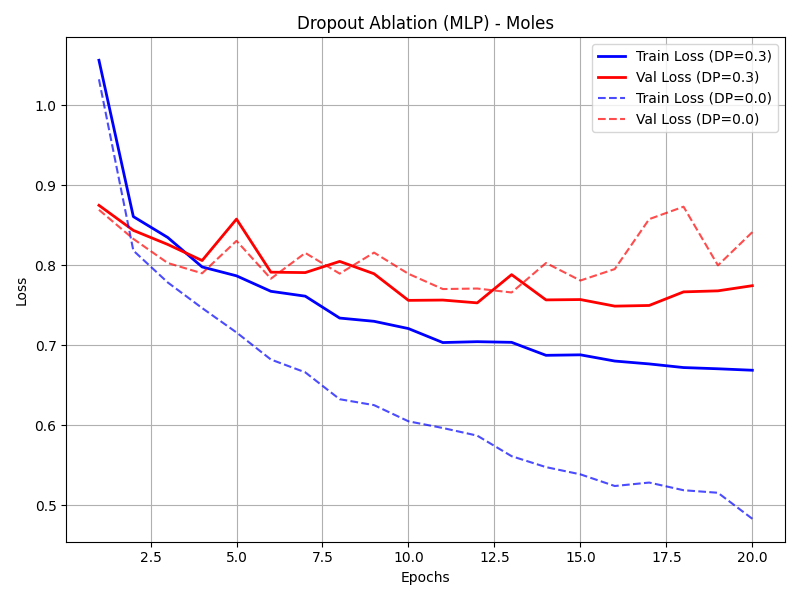
\includegraphics[width=0.48\textwidth]{graphs/mlp_ablation/moles_dropout_ablation.png}
\hfill
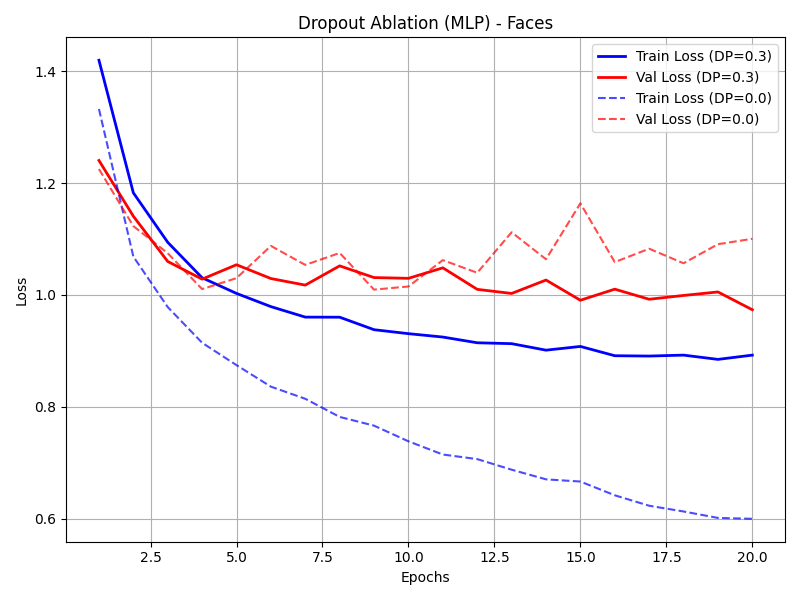
\includegraphics[width=0.48\textwidth]{graphs/mlp_ablation/faces_dropout_ablation.png}
\caption{Comparație Train vs Validation Loss (Dropout 0.3 vs 0.0)}
\end{figure}

\textbf{Analiză supra-reglaj (overfitting) / sub-reglaj (underfitting):}\\
Fără dropout ($p=0.0$), se observă un overfitting pronunțat: funcția de cost pe train scade rapid, iar decalajul (gap-ul) dintre acuratețea de antrenare și cea de validare depășește $10\%$. Introducerea stratului de dropout ($p=0.3$) reduce acest decalaj la $\sim 2\%$, îmbunătățind capacitatea de generalizare a modelului pe ambele seturi de date.

\section{Arhitectura CNN}

\subsection{Descrierea Arhitecturii și a Metodei de Antrenare}
Arhitectura rețelei convoluționale (CNN) a fost concepută pentru a fi comună ambelor seturi de date, respectând restricțiile impuse:
\begin{itemize}
    \item \textbf{Partea convoluțională (4 straturi):}
    \begin{itemize}
        \item \textbf{Stratul 1:} \texttt{Conv2d} ($3 \rightarrow 32$ canale). S-a utilizat un kernel de $3\times3$ (cu pasul/stride 1) pentru datasetul \texttt{Faces} și un kernel de $5\times5$ (sau două straturi succesive de $3\times3$) pentru \texttt{Moles} pentru a mări câmpul receptiv. Urmează \texttt{BatchNorm2d}, \texttt{ReLU} și \texttt{MaxPool2d(2)}.
        \item \textbf{Stratul 2:} \texttt{Conv2d} ($32 \rightarrow 64$ canale, kernel $3\times3$), urmat de \texttt{BatchNorm2d}, \texttt{ReLU} și \texttt{MaxPool2d(2)}.
        \item \textbf{Stratul 3:} \texttt{Conv2d} ($64 \rightarrow 128$ canale, kernel $3\times3$), urmat de \texttt{BatchNorm2d}, \texttt{ReLU} și \texttt{MaxPool2d(2)}.
        \item \textbf{Stratul 4:} \texttt{Conv2d} ($128 \rightarrow 256$ canale, kernel $3\times3$), urmat de \texttt{BatchNorm2d} și \texttt{ReLU}.
        \item Reducerea finală a dimensionalității prin pooling global cu stratul \texttt{AdaptiveAvgPool2d}.
    \end{itemize}
    \item \textbf{Partea de clasificare (2 straturi liniare):}
    \begin{itemize}
        \item Strat liniar ascuns ($256 \rightarrow 128$ neuroni) cu activare \texttt{ReLU} și \texttt{Dropout} ($p=0.3$).
        \item Strat liniar de ieșire ($128 \rightarrow 7$ neuroni).
    \end{itemize}
\end{itemize}
Antrenarea s-a realizat timp de 20 de epoci folosind optimizatorul Adam (learning rate inițial $1e-3$, weight decay $1e-4$) și funcția de cost \texttt{CrossEntropyLoss}, cu un batch size de 64. Rata de învățare a fost menținută constantă ($1e-3$) pe tot parcursul celor 20 de epoci (learning rate scheduling constant).

\section{Comparație Directă Baseline (MLP vs CNN)}
S-a efectuat o analiză comparativă între modelul MLP și modelul CNN pe setul de date \texttt{Moles}, utilizând configurațiile de bază (fără augmentare și fără echilibrarea claselor).

\begin{table}[h!]
\centering
\begin{tabular}{lcc}
\toprule
\textbf{Metrică} & \textbf{CNN Baseline} & \textbf{MLP Baseline} \\
\midrule
Val Acc / F1-micro & \textbf{0.7534} & 0.7384 \\
F1-macro final & \textbf{0.4624} & 0.4242 \\
\bottomrule
\end{tabular}
\caption{Comparație MLP vs CNN pe setul Moles (baseline, fără augmentări)}
\end{table}

\begin{figure}[h!]
\centering
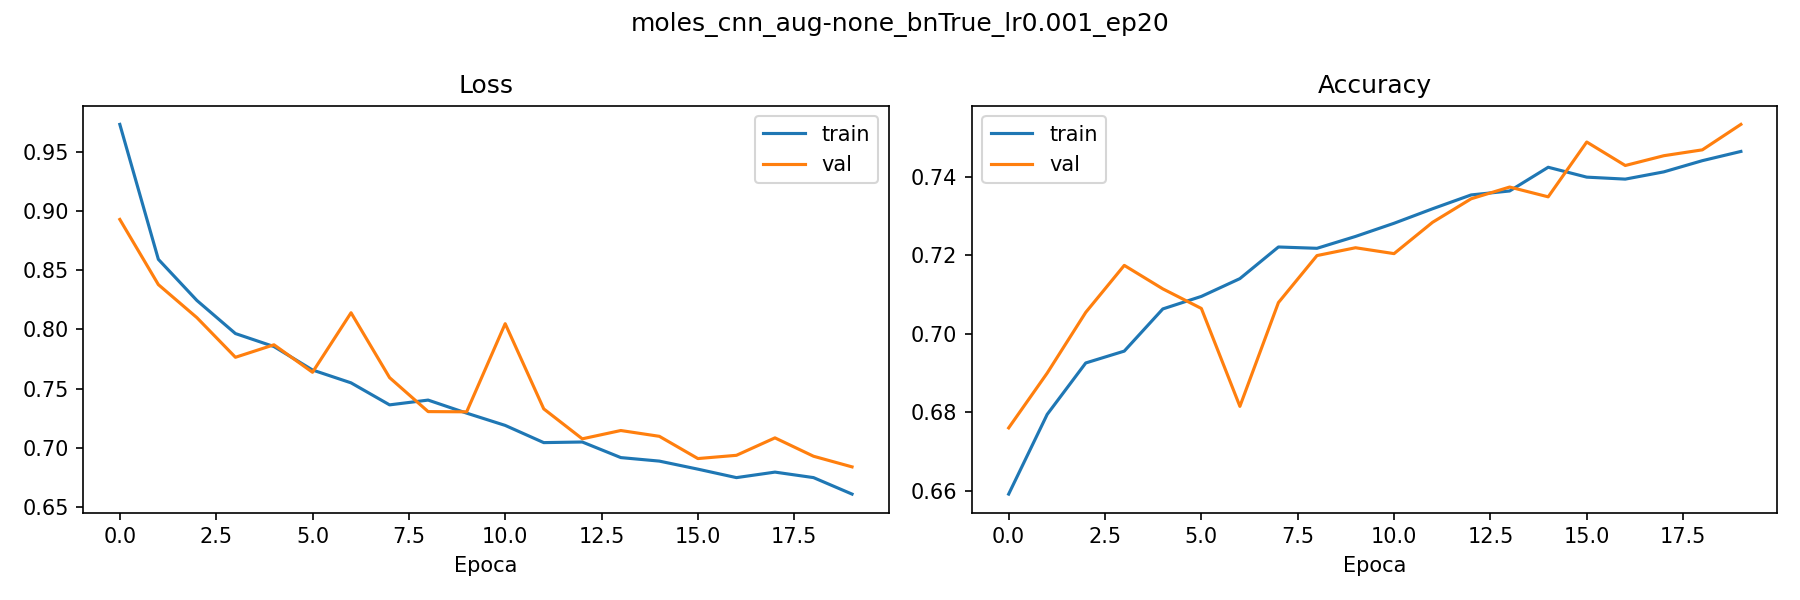
\includegraphics[width=0.8\textwidth]{graphs/cnn_baseline/moles_history.png}
\caption{Grafic antrenare pentru CNN Baseline pe Moles}
\end{figure}

\textbf{Analiză supra-reglaj (overfitting) / sub-reglaj (underfitting):}\\
Modelul CNN Baseline obține o performanță F1-macro superioară modelului MLP ($0.4624$ vs $0.4242$). Cu toate acestea, ambele modele prezintă sub-reglaj pe clasele minoritare (de exemplu, clasa \texttt{df} înregistrează F1-score $0.00$ din cauza numărului extrem de redus de exemple), ceea ce subliniază necesitatea aplicării tehnicilor de echilibrare a datelor.

\section{Ablație CNN: Rolul Batch Normalization}
S-a analizat impactul introducerii straturilor de normalizare pe loturi (\texttt{BatchNorm2d}) în cadrul arhitecturii CNN antrenate timp de 20 de epoci pe setul \texttt{Moles}, comparând:
\begin{enumerate}
    \item \textbf{CNN fără BatchNorm:} Toate straturile convoluționale au \texttt{bias=True} și nu conțin straturi de normalizare.
    \item \textbf{CNN cu BatchNorm:} Straturile convoluționale au \texttt{bias=False}, fiind urmate imediat de \texttt{BatchNorm2d} și de activarea \texttt{ReLU}.
\end{enumerate}

\subsection{Rezultate Comparative}
\begin{table}[h!]
\centering
\begin{tabular}{lcc}
\toprule
\textbf{Configurație CNN} & \textbf{Val Acc / F1-Micro} & \textbf{F1-Macro Final} \\
\midrule
Fără BatchNorm & 0.6695 & 0.1146 \\
\textbf{Cu BatchNorm} & \textbf{0.7534} & \textbf{0.4624} \\
\bottomrule
\end{tabular}
\caption{Comparație performanță globală CNN cu vs fără BatchNorm}
\end{table}

\subsection{Analiza per clasă (F1-Score)}
\begin{table}[h!]
\centering
\begin{tabular}{lccc}
\toprule
\textbf{Clasă} & \textbf{F1-Score (Fără BN)} & \textbf{F1-Score (Cu BN)} & \textbf{Support} \\
\midrule
akiec & 0.00 & \textbf{0.35} & 65 \\
bcc & 0.00 & \textbf{0.52} & 103 \\
bkl & 0.00 & \textbf{0.46} & 220 \\
df & 0.00 & 0.00 & 23 \\
mel & 0.00 & \textbf{0.40} & 222 \\
nv & 0.80 & \textbf{0.88} & 1341 \\
vasc & 0.00 & \textbf{0.63} & 29 \\
\bottomrule
\end{tabular}
\caption{F1-Score pe clase pentru ablația BatchNorm}
\end{table}

\begin{figure}[h!]
\centering
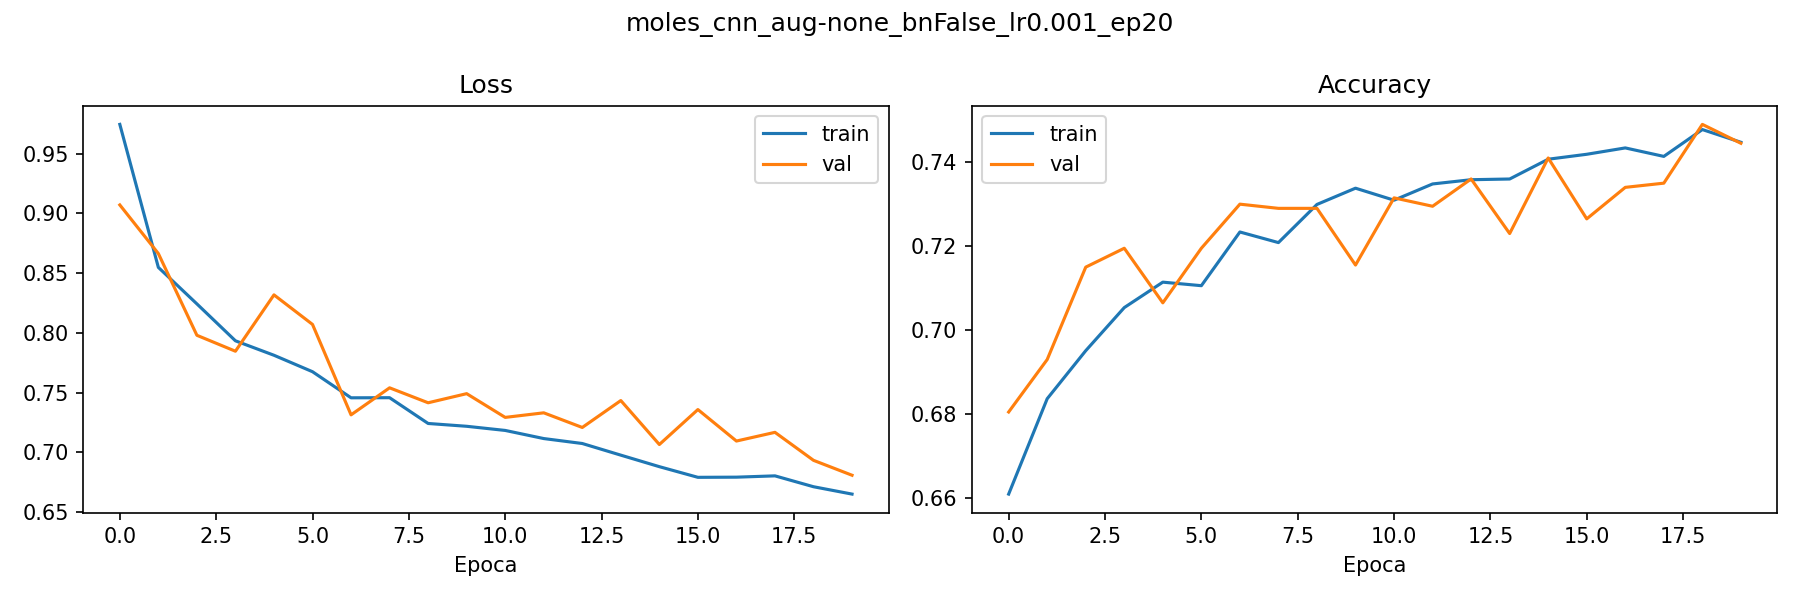
\includegraphics[width=0.48\textwidth]{graphs/norm_ablation/moles_no_bn_history.png}
\hfill
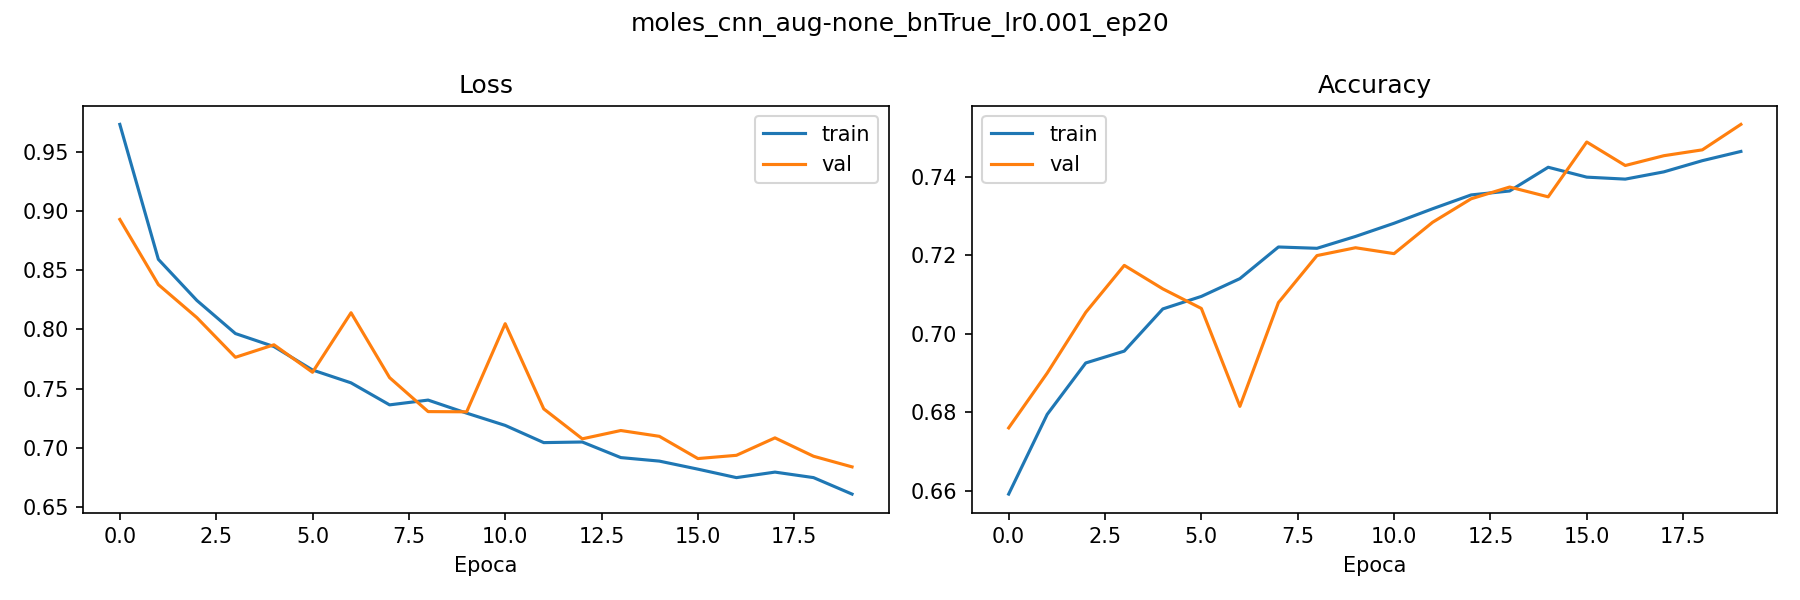
\includegraphics[width=0.48\textwidth]{graphs/norm_ablation/moles_cnn_aug-none_bnTrue_lr0.001_ep20_history.png}
\caption{Curbele de antrenare (Train vs. Test Loss și Performanță) pentru CNN fără BatchNorm (stânga) vs. cu BatchNorm (dreapta) pe Moles}
\label{fig:cnn_bn_ablation}
\end{figure}

\textbf{Analiză supra-reglaj și sub-reglaj (overfit/underfit):}\\
Fără \texttt{BatchNorm2d}, modelul suferă de sub-reglaj sever din cauza instabilității gradienților, obținând un F1-macro de doar $0.1146$ (clasele rare au F1-score zero). Adăugarea normalizării stabilizează antrenarea, crescând F1-macro la $0.4624$, aspect vizibil direct pe curbele de loss și acuratețe din Figura~\ref{fig:cnn_bn_ablation}. Se observă o îmbunătățire semnificativă pe clasele minoritare (de exemplu, F1-score pentru \texttt{mel} crește la $0.40$, iar pentru \texttt{vasc} la $0.63$).

\section{Ablație CNN: Augmentarea Datelor}
S-a evaluat impactul diferitelor scheme de augmentare aplicate modelului CNN (cu BatchNorm) pe parcursul a 20 de epoci pe setul \texttt{Moles}:
\begin{itemize}
    \item \texttt{none}: Doar redimensionare și normalizare (baseline).
    \item \texttt{geometric}: Rotații aleatoare (maxim $15^\circ$), decupare aleatoare (crop) și reflexie orizontală (flip).
    \item \texttt{color}: Modificări de contrast, luminozitate și saturație prin \texttt{ColorJitter}.
    \item \texttt{all}: Combinarea augmentărilor geometrice cu cele de culoare.
\end{itemize}

\begin{figure}[h!]
\centering
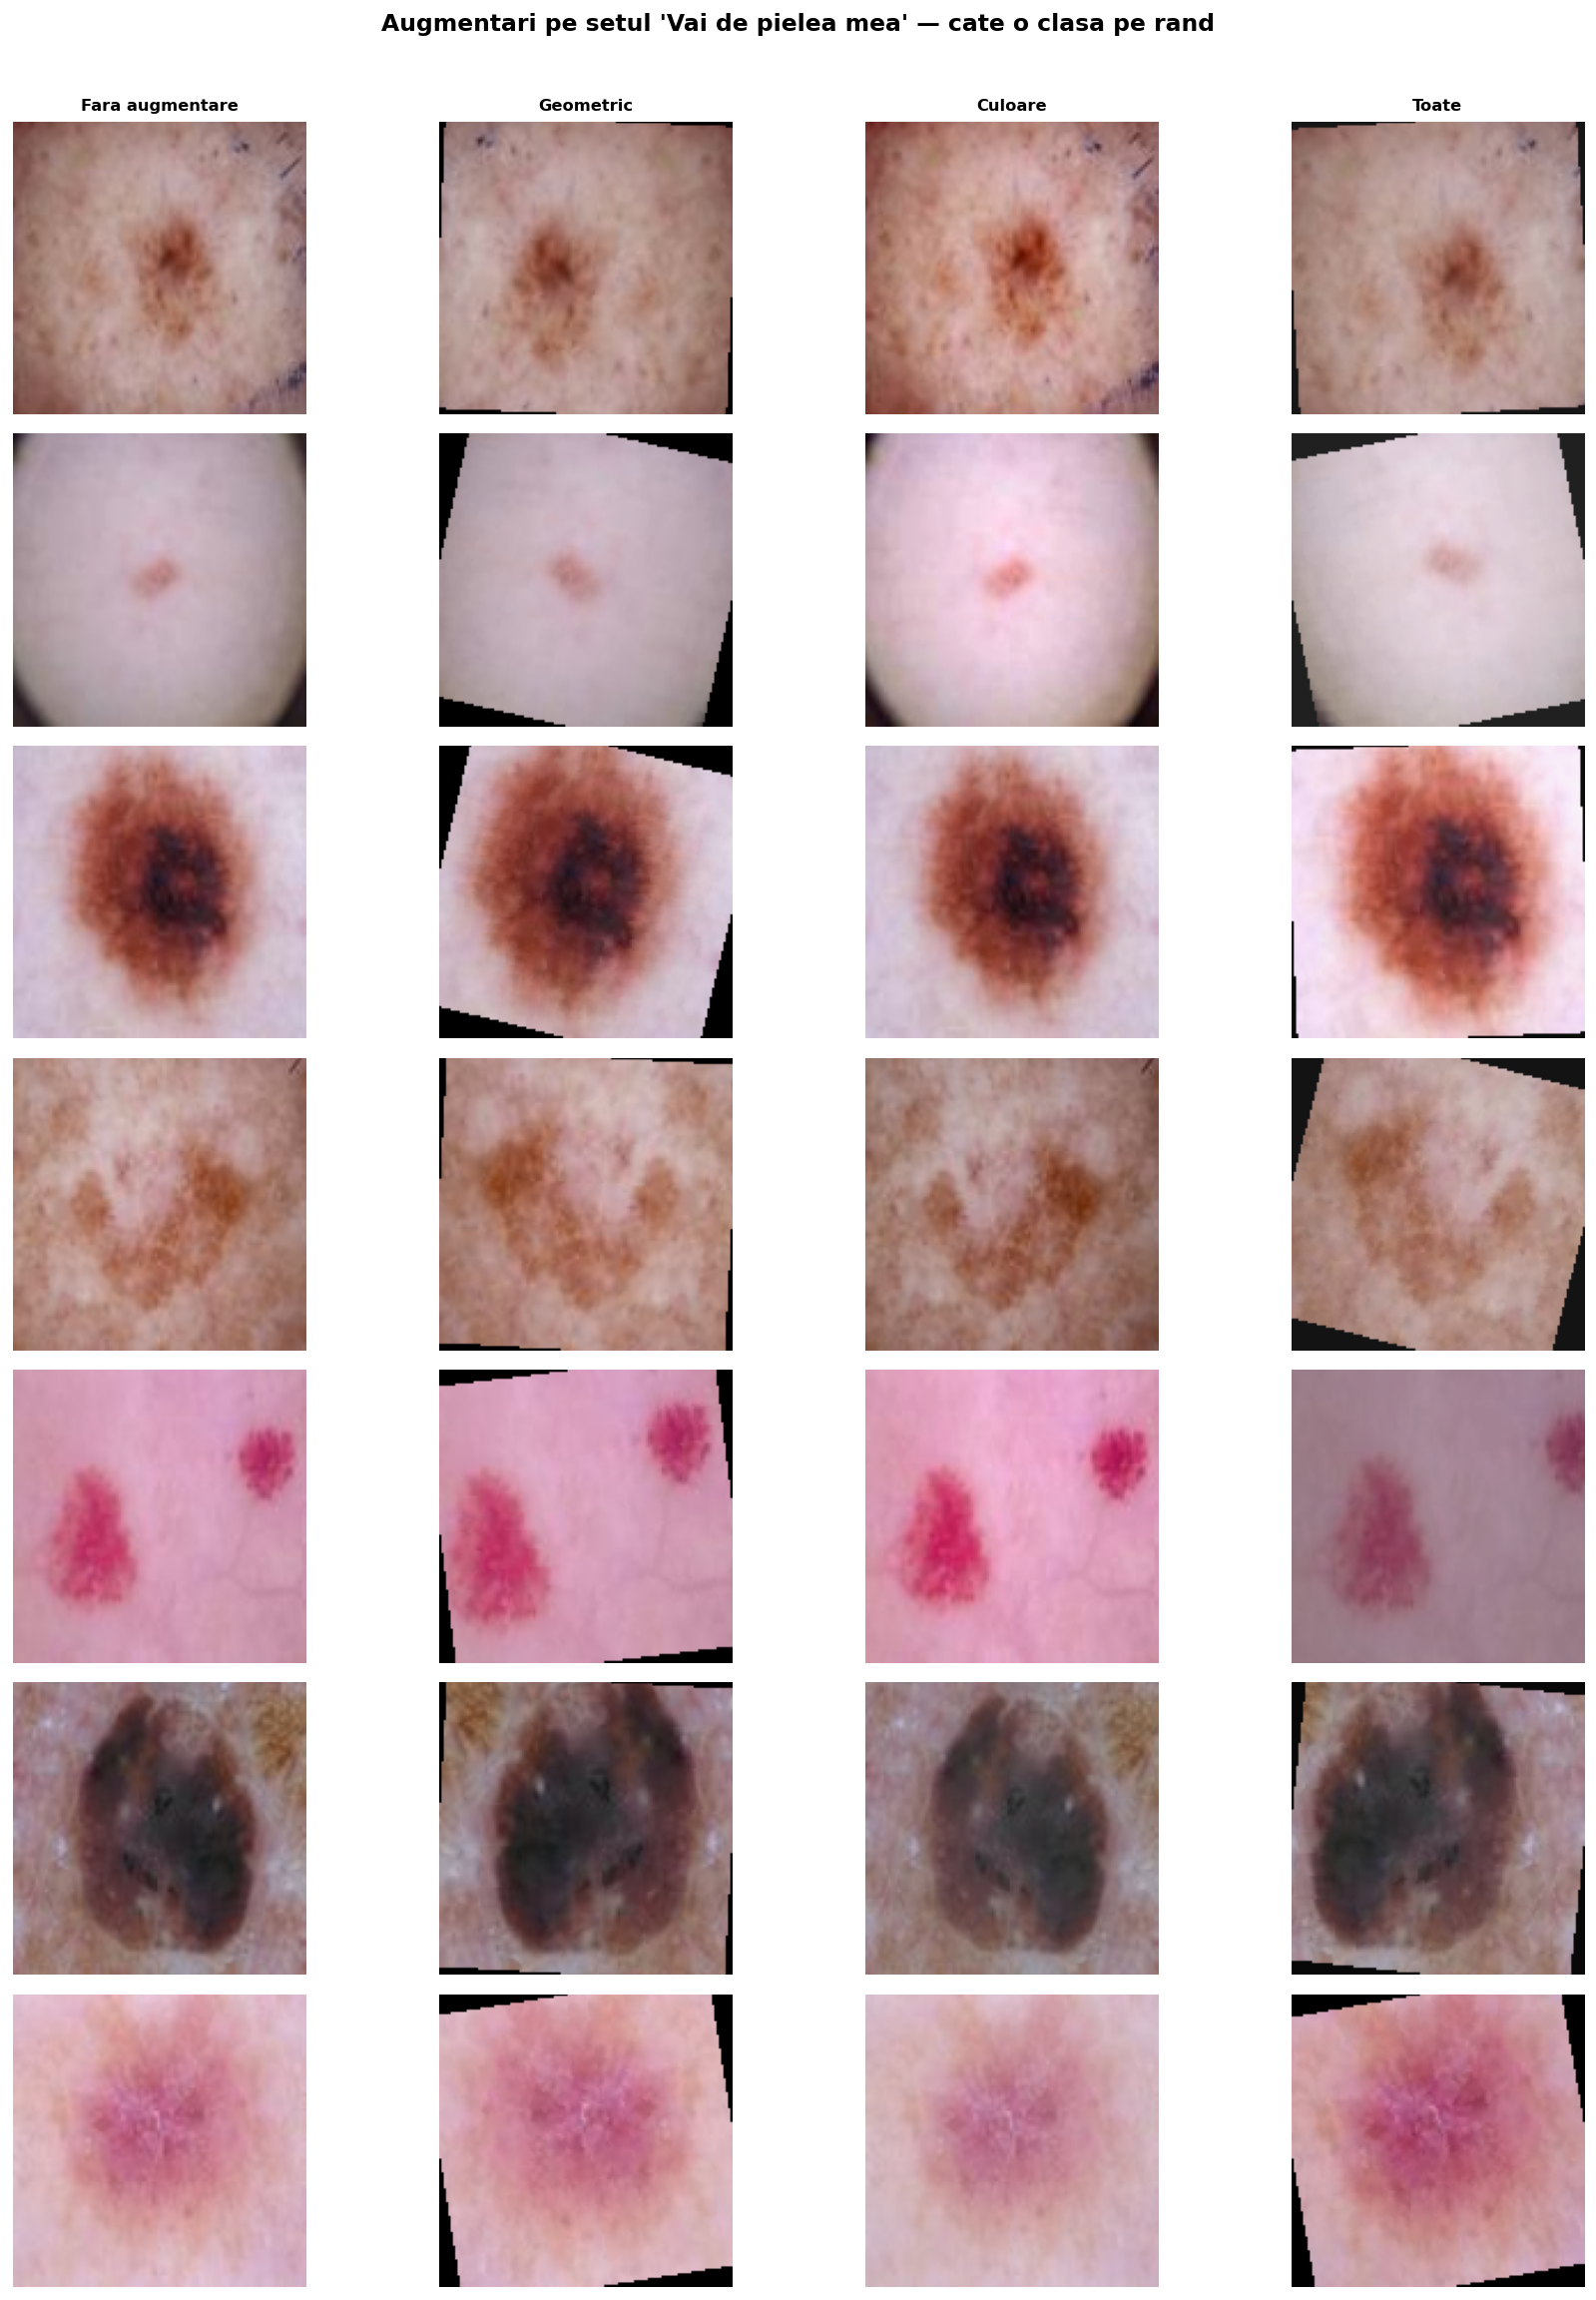
\includegraphics[width=0.8\textwidth]{graphs/aug_ablation/moles_demo.png}
\caption{Exemple de augmentări pe setul Moles}
\end{figure}

\subsection{Rezultate Comparative}
\begin{table}[h!]
\centering
\begin{tabular}{lcc}
\toprule
\textbf{Configurație Augmentare} & \textbf{Val Acc / F1-Micro} & \textbf{F1-Macro} \\
\midrule
Fără augmentări (\texttt{none}) & \textbf{0.7534} & \textbf{0.4624} \\
Geometric (\texttt{geometric}) & 0.7434 & 0.4483 \\
Culoare (\texttt{color}) & 0.7374 & 0.4430 \\
Toate (\texttt{all}) & 0.7424 & 0.4233 \\
\bottomrule
\end{tabular}
\caption{Efectul diferitelor tipuri de augmentări (20 epoci)}
\end{table}

\begin{figure}[h!]
\centering
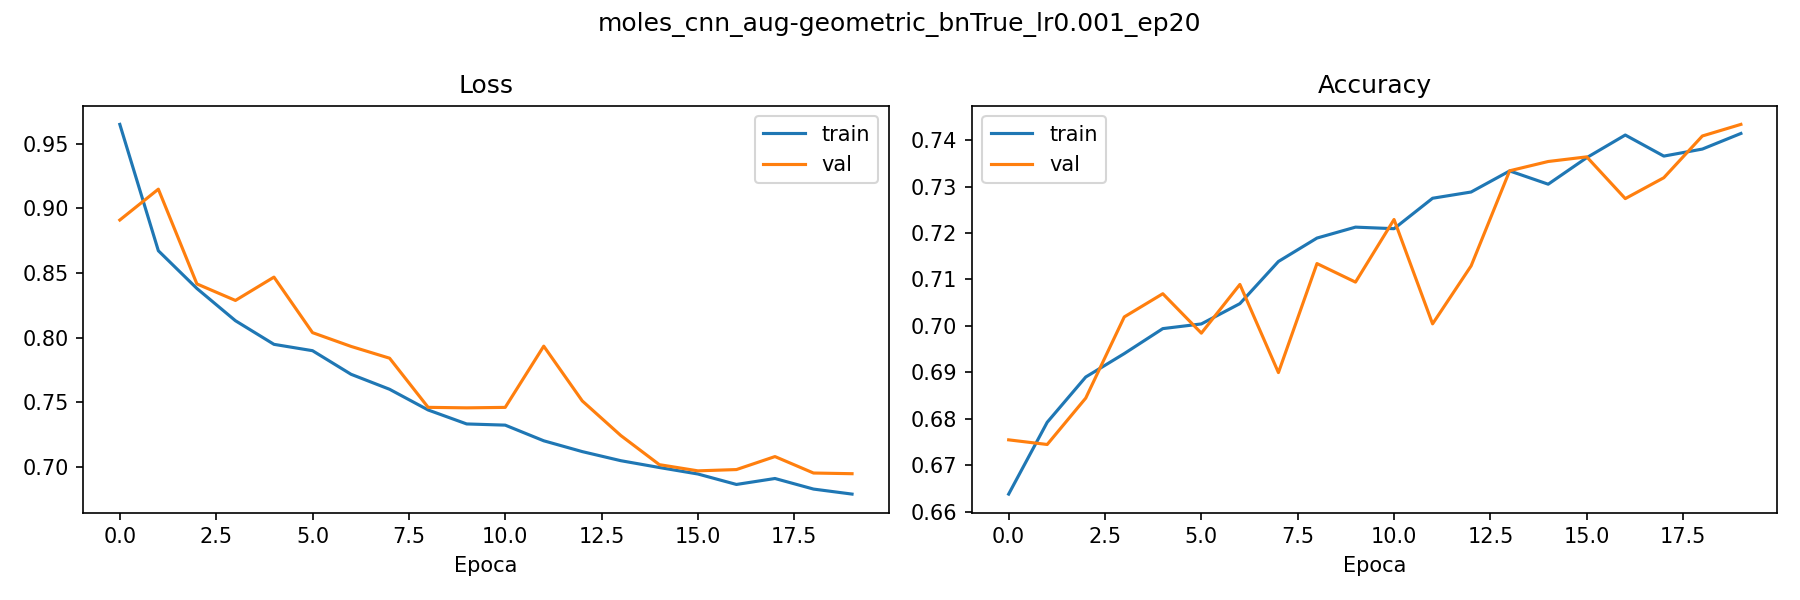
\includegraphics[width=0.32\textwidth]{graphs/aug_ablation/moles_cnn_aug-geometric_bnTrue_lr0.001_ep20_history.png}
\hfill
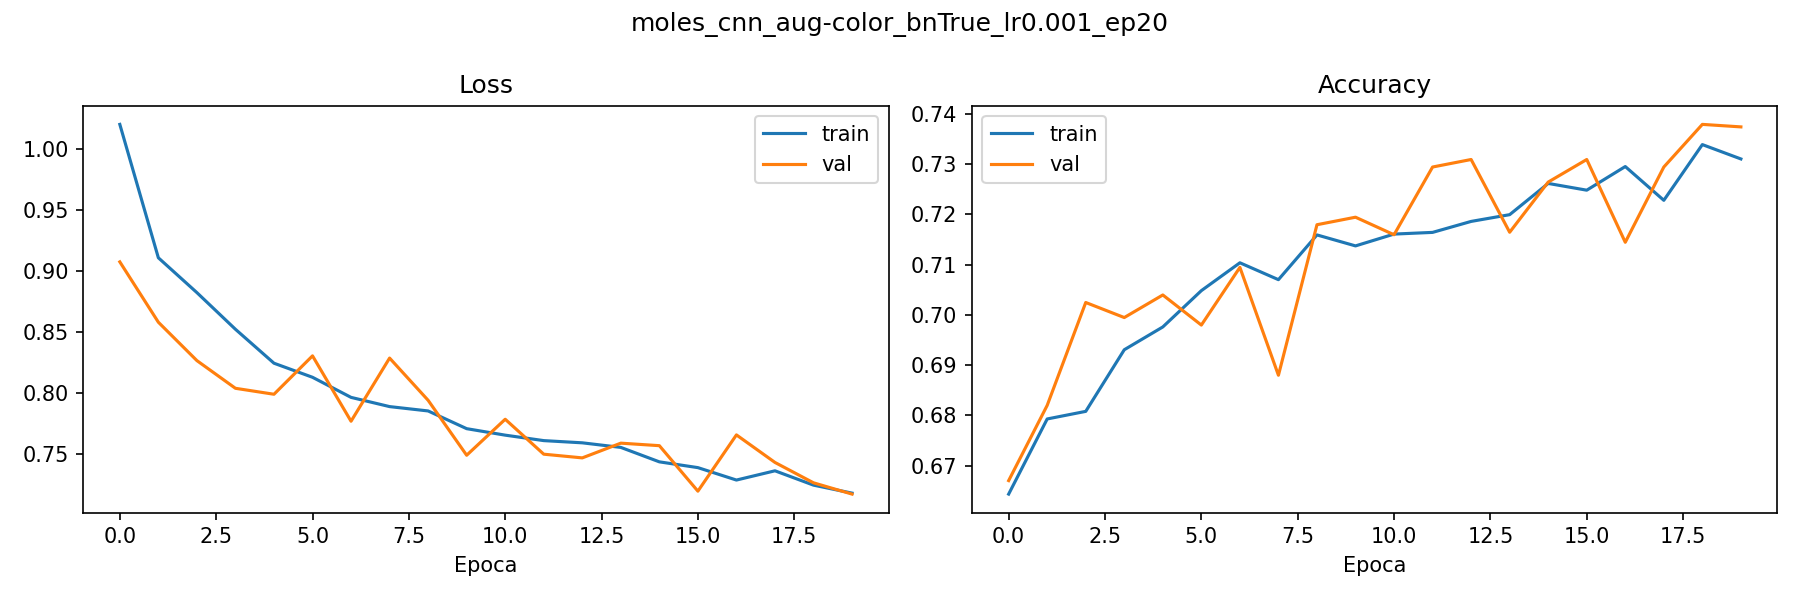
\includegraphics[width=0.32\textwidth]{graphs/aug_ablation/moles_cnn_aug-color_bnTrue_lr0.001_ep20_history.png}
\hfill
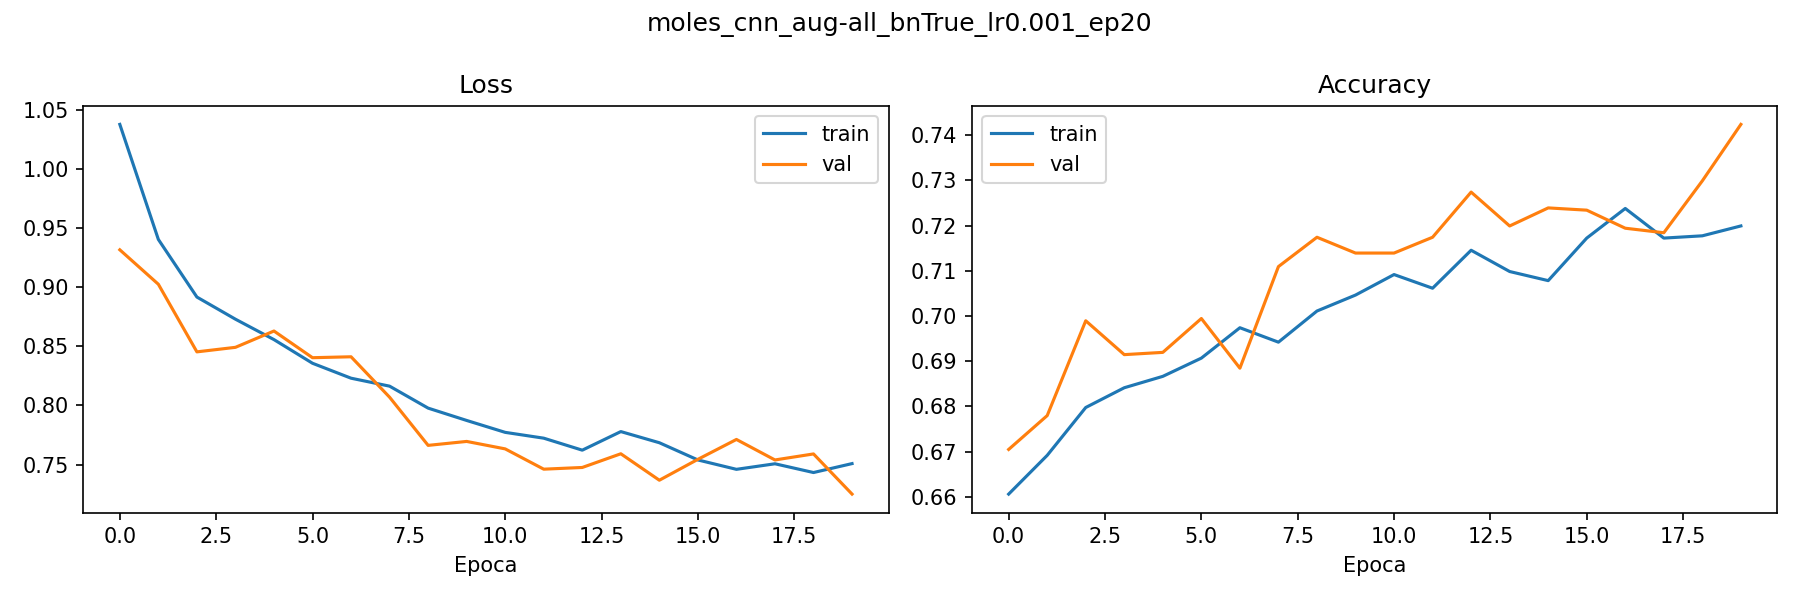
\includegraphics[width=0.32\textwidth]{graphs/aug_ablation/moles_cnn_aug-all_bnTrue_lr0.001_ep20_history.png}
\caption{Curbele de antrenare pentru configurațiile de augmentare pe Moles: Geometric (stânga), Color (mijloc) și All (dreapta)}
\label{fig:cnn_aug_ablation_moles}
\end{figure}

\textbf{Analiză supra-reglaj și sub-reglaj (overfit/underfit):}\\
În absența augmentării (configurația \texttt{none}), se observă debutul supra-reglajului (decalaj între pierderea de antrenare și cea de validare). Aplicarea schemelor de augmentare (\texttt{color}, \texttt{all}) reduce acest decalaj, acționând ca regularizare (așa cum se observă din curbele de loss din Figura~\ref{fig:cnn_aug_ablation_moles}). Totuși, performanța F1-macro scade în cele 20 de epoci din cauza sub-reglajului (complexitatea datelor augmentate necesită un număr mai mare de epoci de antrenare pentru convergență).

\section{Particularități pe Setul „You're on Candid Camera” (Faces)}
S-au comparat performanțele modelelor MLP și CNN (cu și fără BatchNorm) antrenate timp de 20 de epoci pe setul \texttt{Faces}, fără augmentări.

\begin{table}[h!]
\centering
\begin{tabular}{lcc}
\toprule
\textbf{Model pe dataset „Faces”} & \textbf{Val Acc / F1-Micro} & \textbf{F1-Macro Val} \\
\midrule
MLP (Dropout 0.3) & 0.6560 & \textbf{0.5253} \\
CNN (Fără BatchNorm) & 0.5128 & 0.2471 \\
CNN (Cu BatchNorm) & \textbf{0.5868} & 0.4229 \\
\bottomrule
\end{tabular}
\caption{Performanța modelelor pe setul cu expresii faciale}
\end{table}

\begin{figure}[h!]
\centering
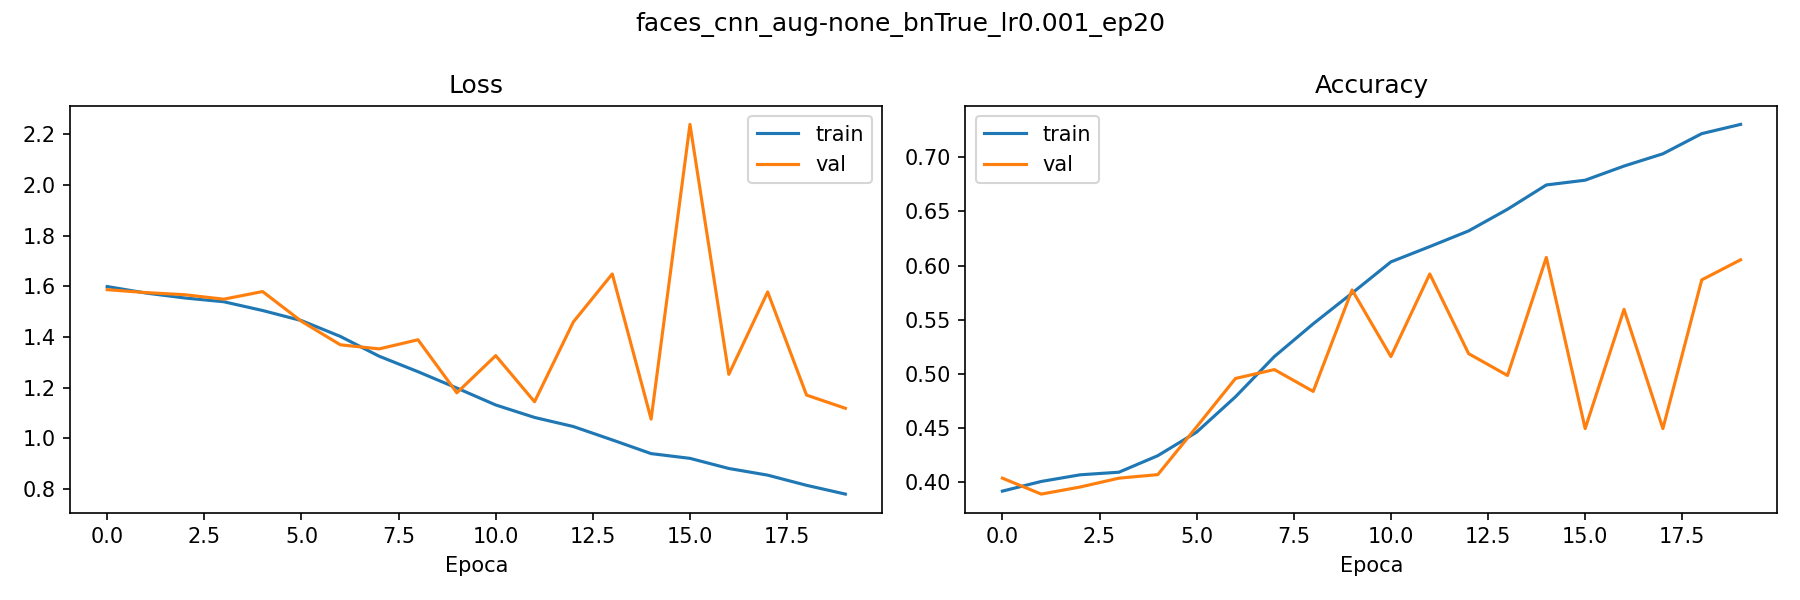
\includegraphics[width=0.8\textwidth]{graphs/cnn_baseline/faces_history.png}
\caption{Grafic antrenare pentru CNN (cu BN) pe Faces}
\end{figure}

\textbf{Analiză supra-reglaj (overfitting) / sub-reglaj (underfitting):}\\
Pe setul \texttt{Faces}, modelul MLP obține performanțe superioare rețelelor convoluționale simple datorită regularizării eficiente prin Dropout ($p=0.3$). Modelul CNN fără BatchNorm suferă de sub-reglaj major (gradient vanishing/exploding), clasificând majoritatea exemplelor în clasa dominantă (\texttt{Happiness}). Introducerea \texttt{BatchNorm} stabilizează modelul și crește F1-macro la $0.4229$.

\subsection{Ablația Augmentărilor pe CNN (cu BatchNorm) la Faces}
S-a analizat impactul aceleiași scheme de augmentare pe setul \texttt{Faces}:

\begin{figure}[h!]
\centering
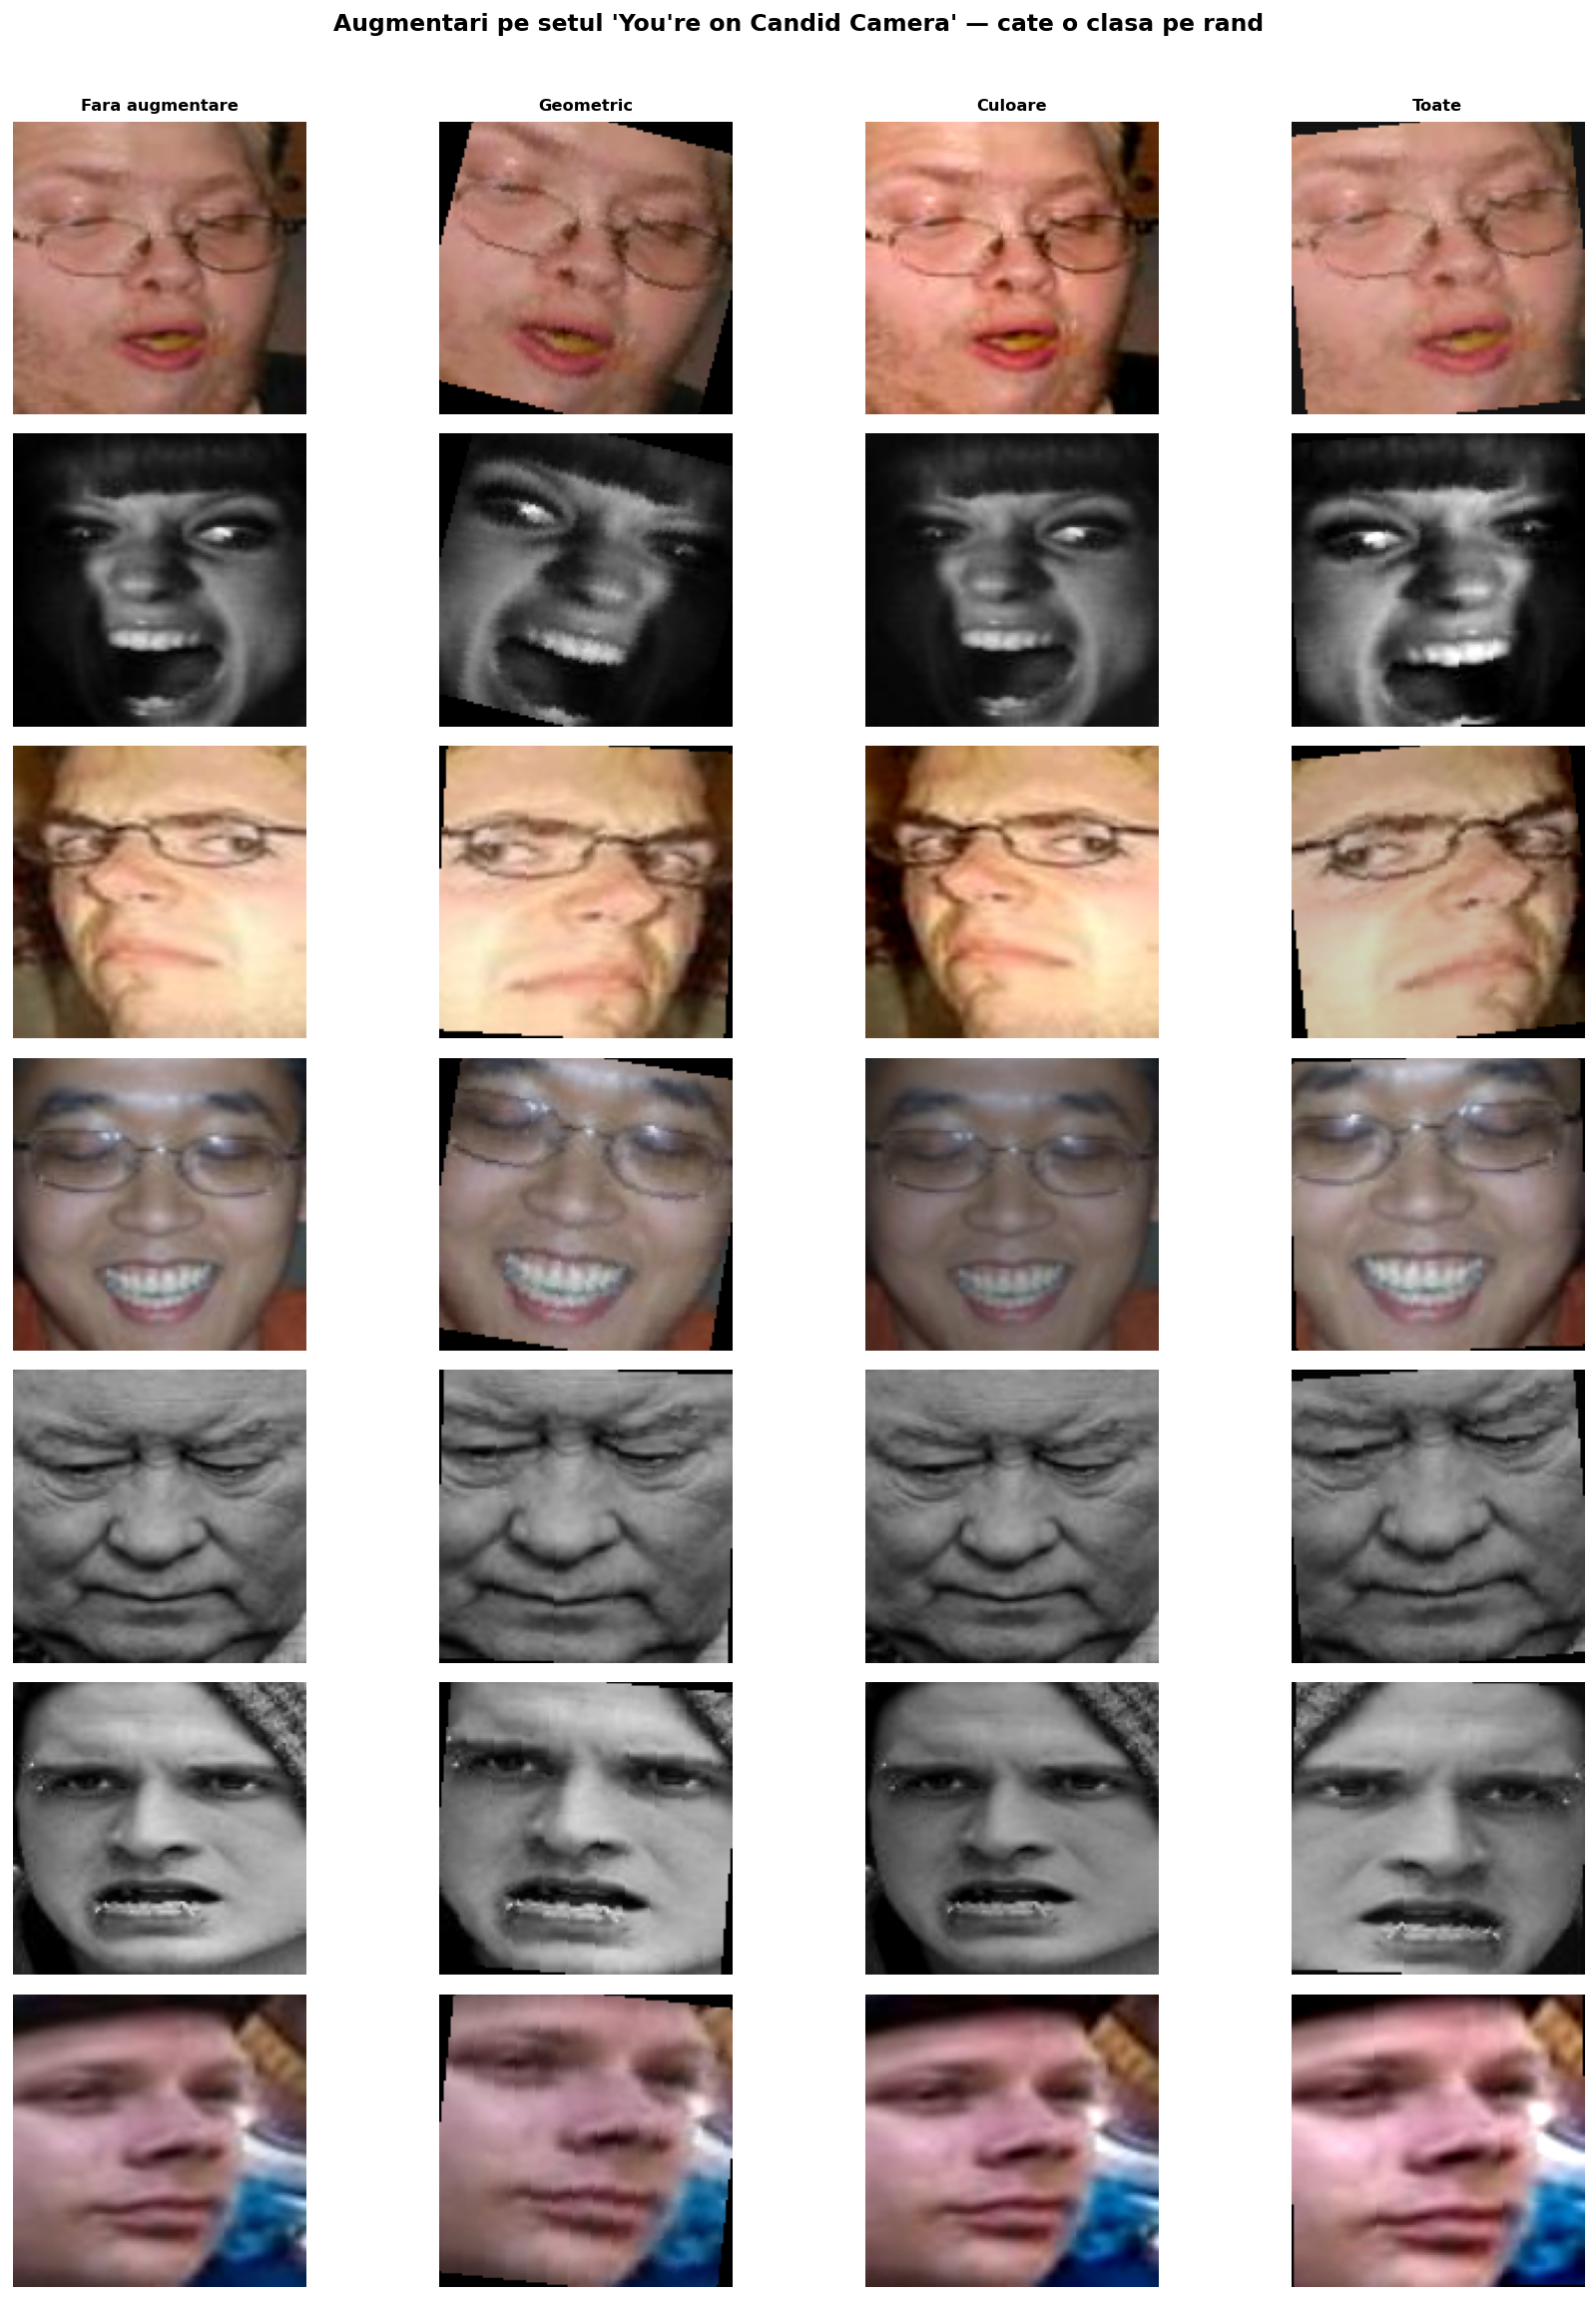
\includegraphics[width=0.8\textwidth]{graphs/aug_ablation/faces_demo.png}
\caption{Exemple de augmentări pe setul Faces}
\end{figure}

\begin{table}[h!]
\centering
\begin{tabular}{lcc}
\toprule
\textbf{Configurație} & \textbf{Val Acc / F1-Micro} & \textbf{F1-Macro Val} \\
\midrule
Fără augmentări (\texttt{none}) & 0.5868 & 0.4229 \\
Geometric (\texttt{geometric}) & 0.6042 & \textbf{0.4532} \\
Culoare (\texttt{color}) & \textbf{0.6157} & 0.4212 \\
Toate (\texttt{all}) & 0.5836 & 0.3626 \\
\bottomrule
\end{tabular}
\caption{Rezultate augmentări pe expresii faciale}
\end{table}

\begin{figure}[h!]
\centering
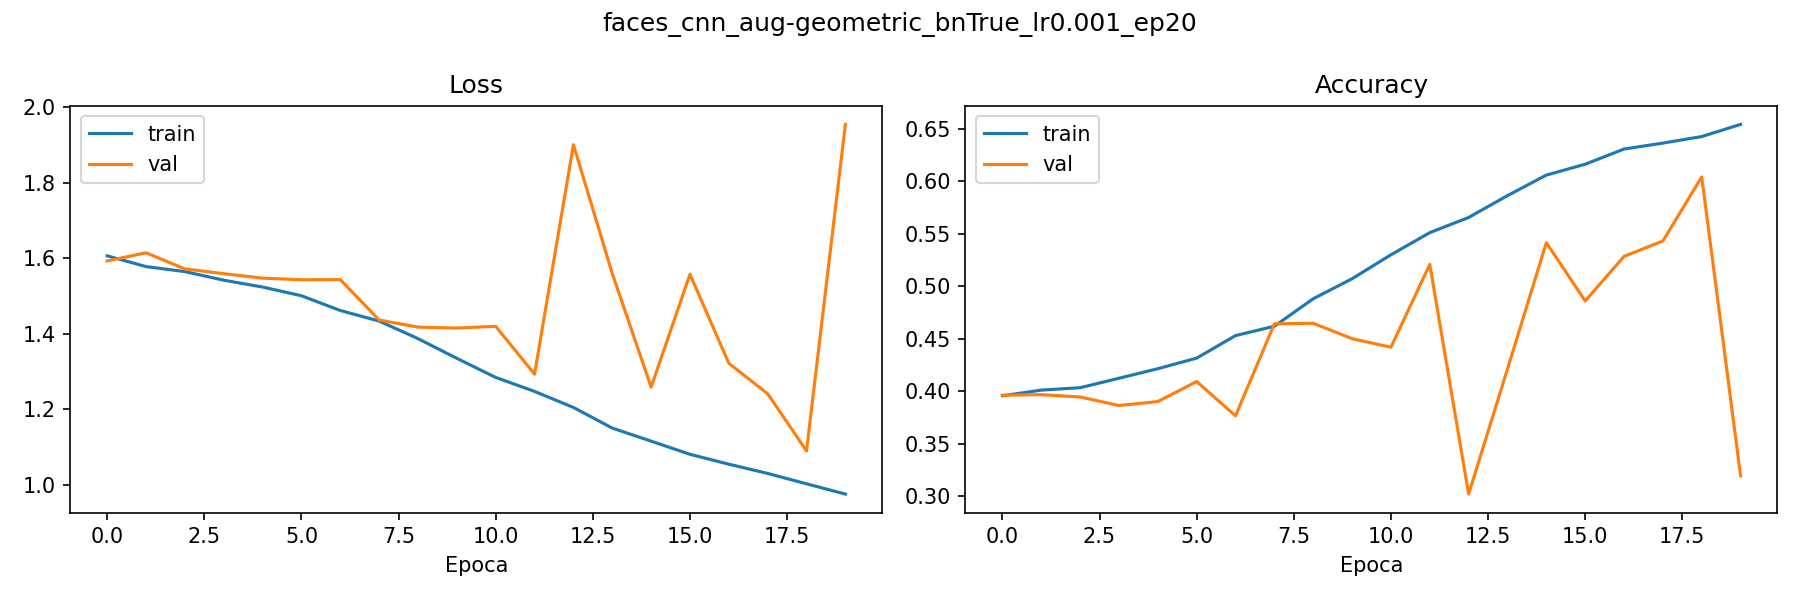
\includegraphics[width=0.32\textwidth]{graphs/aug_ablation/faces_cnn_aug-geometric_bnTrue_lr0.001_ep20_history.png}
\hfill
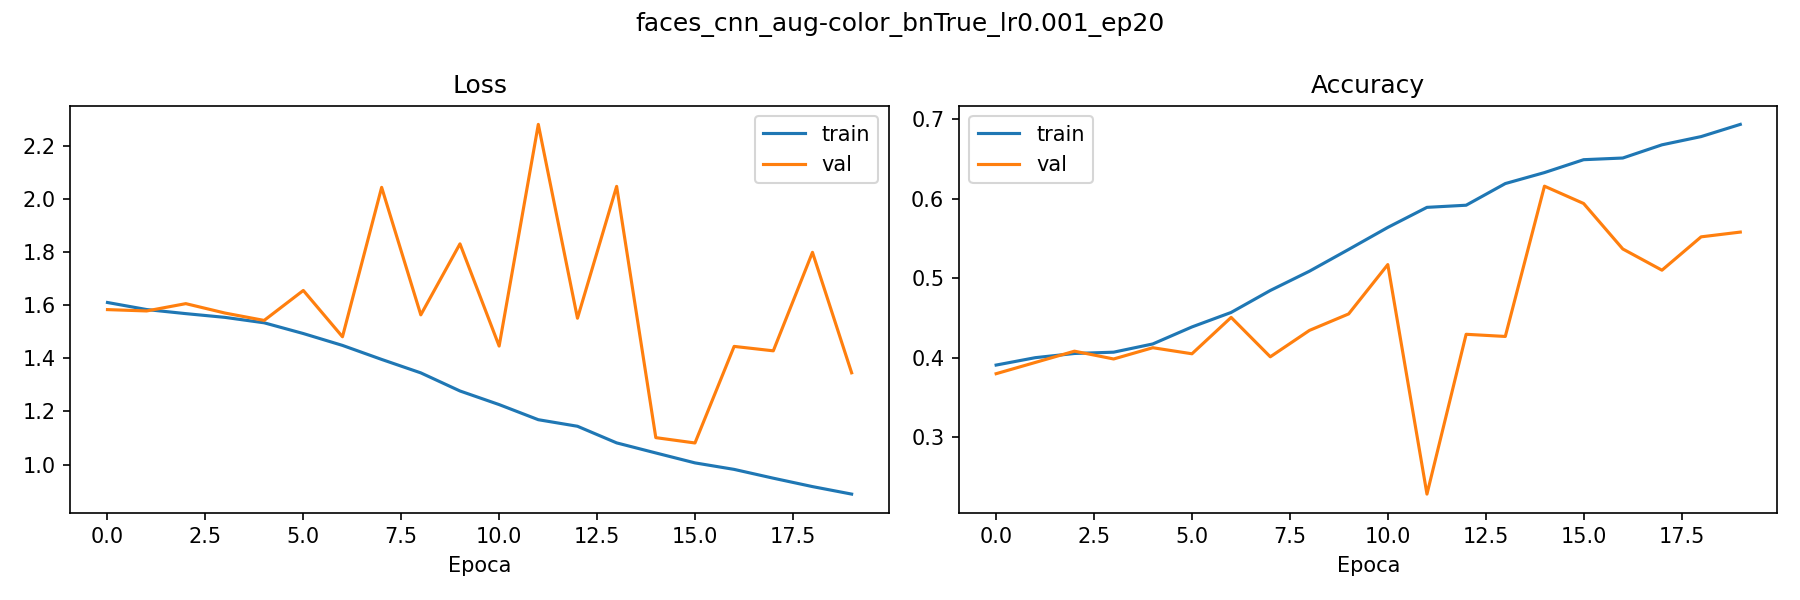
\includegraphics[width=0.32\textwidth]{graphs/aug_ablation/faces_cnn_aug-color_bnTrue_lr0.001_ep20_history.png}
\hfill
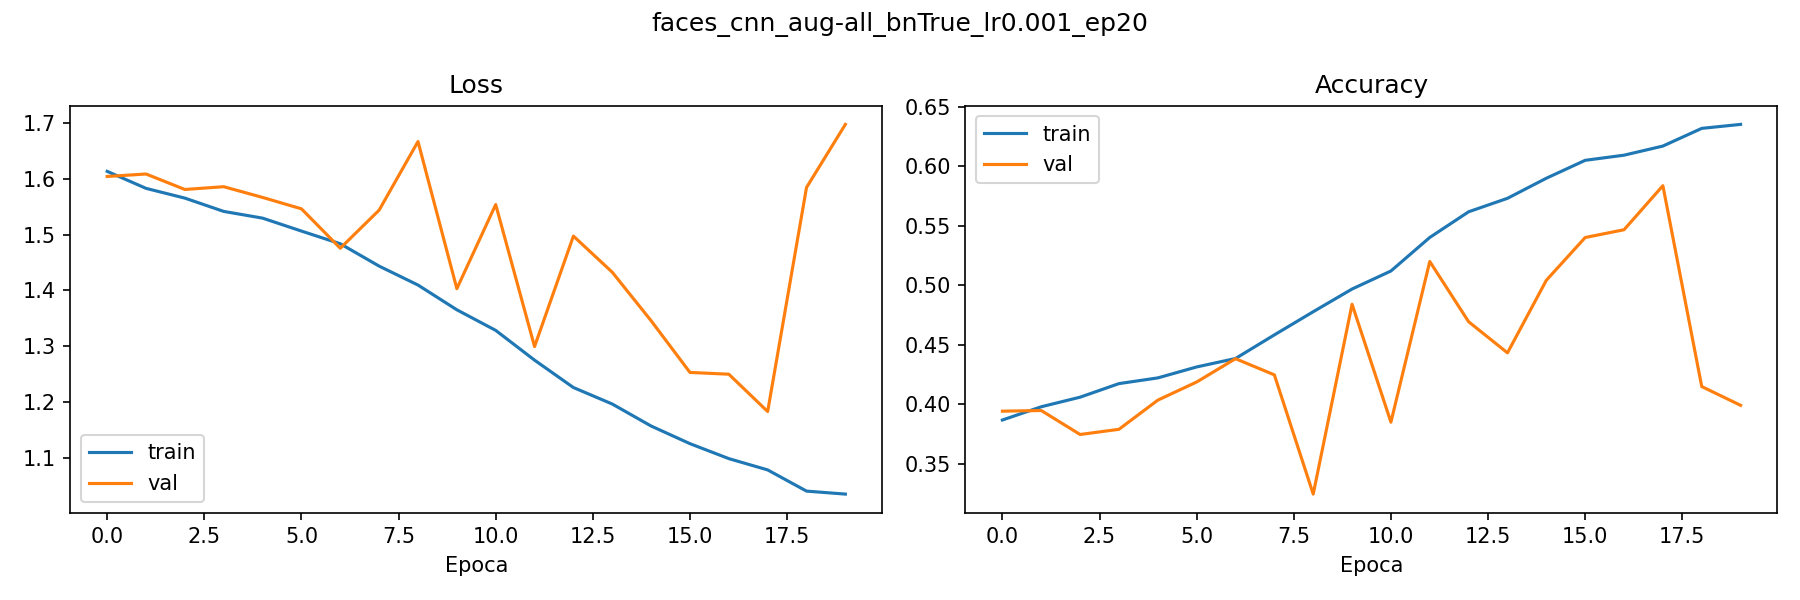
\includegraphics[width=0.32\textwidth]{graphs/aug_ablation/faces_cnn_aug-all_bnTrue_lr0.001_ep20_history.png}
\caption{Curbele de antrenare pentru configurațiile de augmentare pe Faces: Geometric (stânga), Color (mijloc) și All (dreapta)}
\label{fig:cnn_aug_ablation_faces}
\end{figure}

\textbf{Analiză supra-reglaj și sub-reglaj (overfit/underfit):}\\
Augmentările geometrice și cele de culoare oferă o ușoară îmbunătățire a generalizării în cele 20 de epoci (F1-macro crește la $0.4532$ pentru geometric, curbele putând fi analizate comparativ în Figura~\ref{fig:cnn_aug_ablation_faces}). Combinarea tuturor augmentărilor (\texttt{all}) duce la un debut de sub-reglaj (F1-macro scade la $0.3626$), zgomotul suplimentar introdus necesitând un timp de antrenare mai lung pentru adaptare.

\section{Tratarea Dezechilibrului de Clase (Ablații)}
S-au evaluat trei strategii de combatere a dezechilibrului claselor, utilizând modelul CNN (cu BatchNorm) antrenat timp de 20 de epoci fără augmentări:
\begin{itemize}
    \item \texttt{none}: Antrenare standard fără corecții (baseline).
    \item \texttt{weighted\_ce}: Ponderarea funcției de cost: $w_c = \frac{N_{total}}{K \cdot N_c}$.
    \item \texttt{sampler}: Utilizarea unui \texttt{WeightedRandomSampler} în loader pentru supra-eșantionarea (oversampling) claselor minoritare.
    \item \texttt{focal}: Utilizarea Focal Loss cu pondere $\alpha$ invers proporțională și $\gamma=2.0$ pentru a prioritiza mostrele dificile.
\end{itemize}

\subsection{Rezultate pe Setul de Alunite (Moles)}
\begin{table}[h!]
\centering
\setlength{\tabcolsep}{4pt}
\makebox[\textwidth][c]{
\begin{tabular}{lccccc}
\toprule
\textbf{Strategie} & \textbf{Acc / F1-micro} & \textbf{F1-macro} & \textbf{Rec. df} & \textbf{Rec. mel} & \textbf{Rec. vasc} \\
\midrule
Baseline (\texttt{none}) & \textbf{0.7534} & 0.4624 & 0.00 & 0.32 & 0.55 \\
Weighted CE & 0.5731 & 0.4194 & 0.17 & \textbf{0.69} & \textbf{0.90} \\
\textbf{Weighted Sampler} & 0.6430 & \textbf{0.4975} & \textbf{0.48} & 0.52 & 0.86 \\
Focal Loss & 0.4408 & 0.3628 & 0.30 & 0.48 & 0.79 \\
\bottomrule
\end{tabular}
}
\caption{Ablație imbalance pe setul Moles}
\end{table}

\textbf{Analiză supra-reglaj (overfitting) / sub-reglaj (underfitting):}\\
\texttt{WeightedRandomSampler} oferă cele mai bune performanțe pe setul \texttt{Moles}, crescând F1-macro la $0.4975$ și reactivând clasa extrem de rară \texttt{df} (recall $0.48$, față de $0.00$ la baseline). \texttt{Weighted CE} îmbunătățește sensibilitatea claselor minoritare (\texttt{mel} recall $0.69$, \texttt{vasc} recall $0.90$), dar induce un sub-reglaj pe clasa majoritară \texttt{nv}, scăzând acuratețea globală la $57.3\%$. Focal Loss obține rezultate slabe ($0.3628$ F1-macro) din cauza dificultății de convergență în 20 de epoci.

\begin{figure}[h!]
\centering
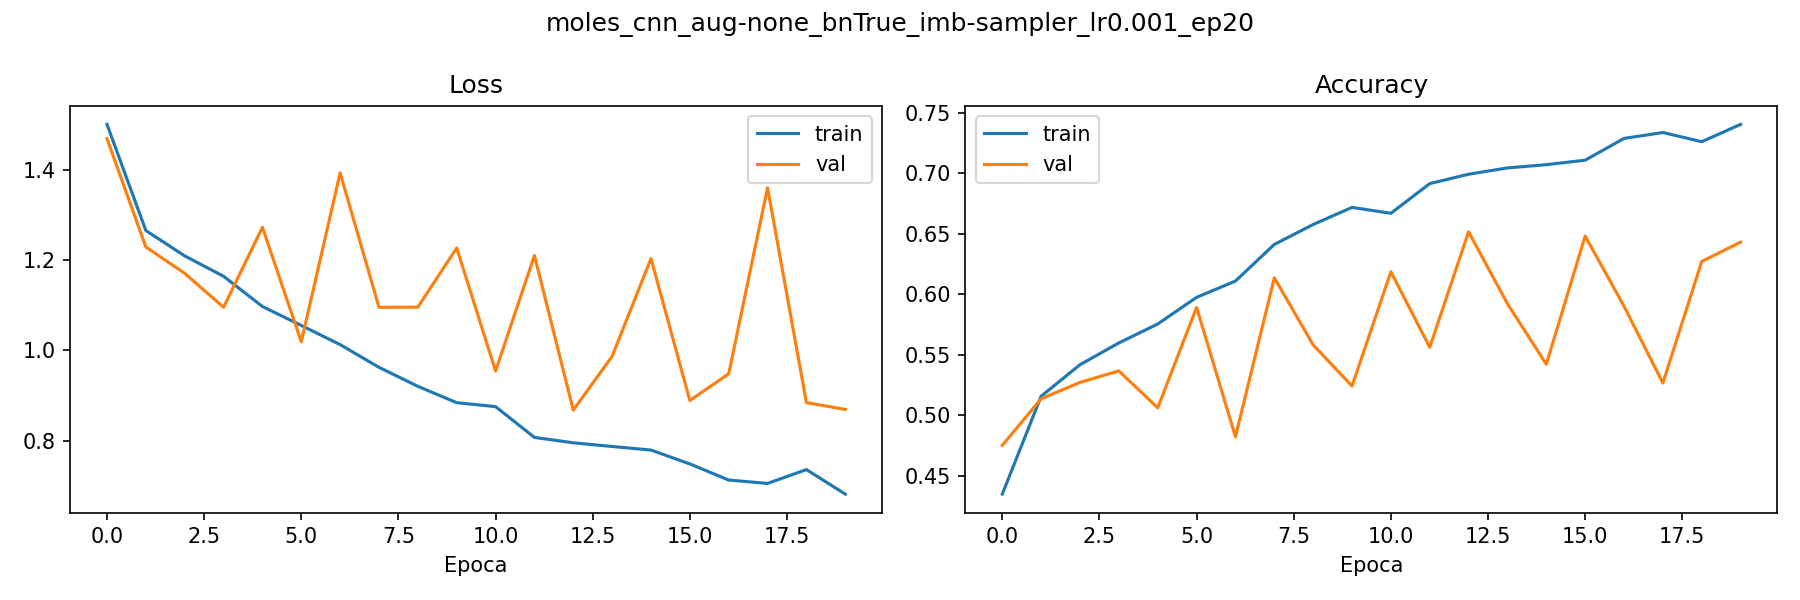
\includegraphics[width=0.48\textwidth]{graphs/imbalance_ablation/moles_sampler_history.png}
\hfill
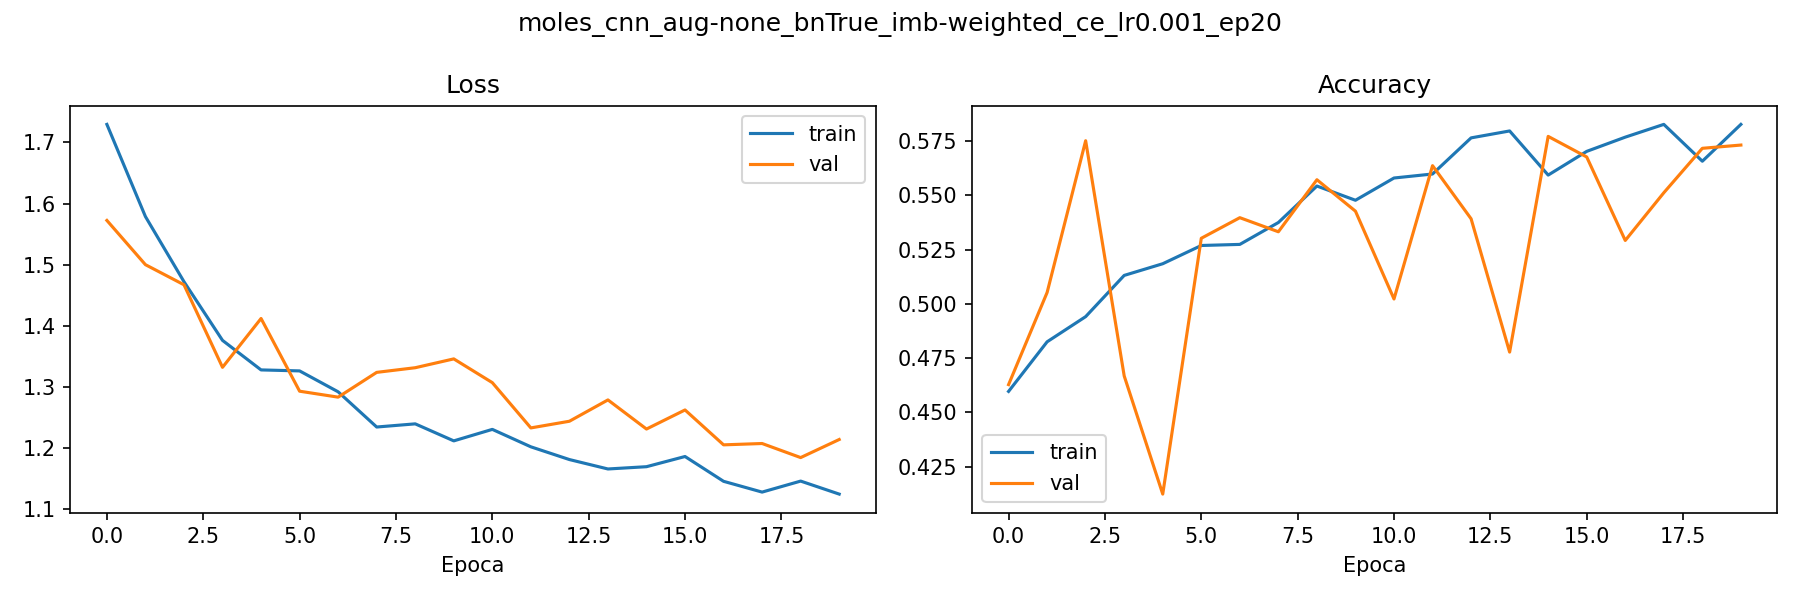
\includegraphics[width=0.48\textwidth]{graphs/imbalance_ablation/moles_weighted_ce_history.png}
\caption{Istoricul antrenării pe Moles cu tehnici de echilibrare: Weighted Random Sampler (stânga) și Weighted Cross Entropy (dreapta)}
\end{figure}

\subsection{Rezultate pe Setul de Expresii Faciale (Faces)}
\begin{table}[h!]
\centering
\setlength{\tabcolsep}{4pt}
\makebox[\textwidth][c]{
\begin{tabular}{lccccc}
\toprule
\textbf{Strategie} & \textbf{Acc / F1-micro} & \textbf{F1-macro} & \textbf{Rec. Fear} & \textbf{Rec. Disgust} & \textbf{Rec. Anger} \\
\midrule
Baseline (\texttt{none}) & \textbf{0.5868} & 0.4229 & 0.00 & 0.02 & 0.42 \\
Weighted CE & 0.5558 & 0.4004 & 0.26 & 0.07 & 0.21 \\
Weighted Sampler & 0.4997 & \textbf{0.4740} & \textbf{0.43} & \textbf{0.61} & 0.37 \\
Focal Loss & 0.3048 & 0.3028 & 0.52 & 0.30 & \textbf{0.35} \\
\bottomrule
\end{tabular}
}
\caption{Ablație imbalance pe setul Faces}
\end{table}

\textbf{Analiză supra-reglaj (overfitting) / sub-reglaj (underfitting):}\\
Pe setul \texttt{Faces}, \texttt{WeightedRandomSampler} înregistrează cea mai bună performanță F1-macro ($0.4740$), crescând recall-ul pe clasele rare \texttt{Fear} ($0.43$) și \texttt{Disgust} ($0.61$). \texttt{Weighted CE} oferă un compromis bun, menținând acuratețea globală la $55.58\%$, în timp ce Focal Loss prezintă o instabilitate puternică a antrenării (acuratețe globală de doar $30.48\%$).

\begin{figure}[h!]
\centering
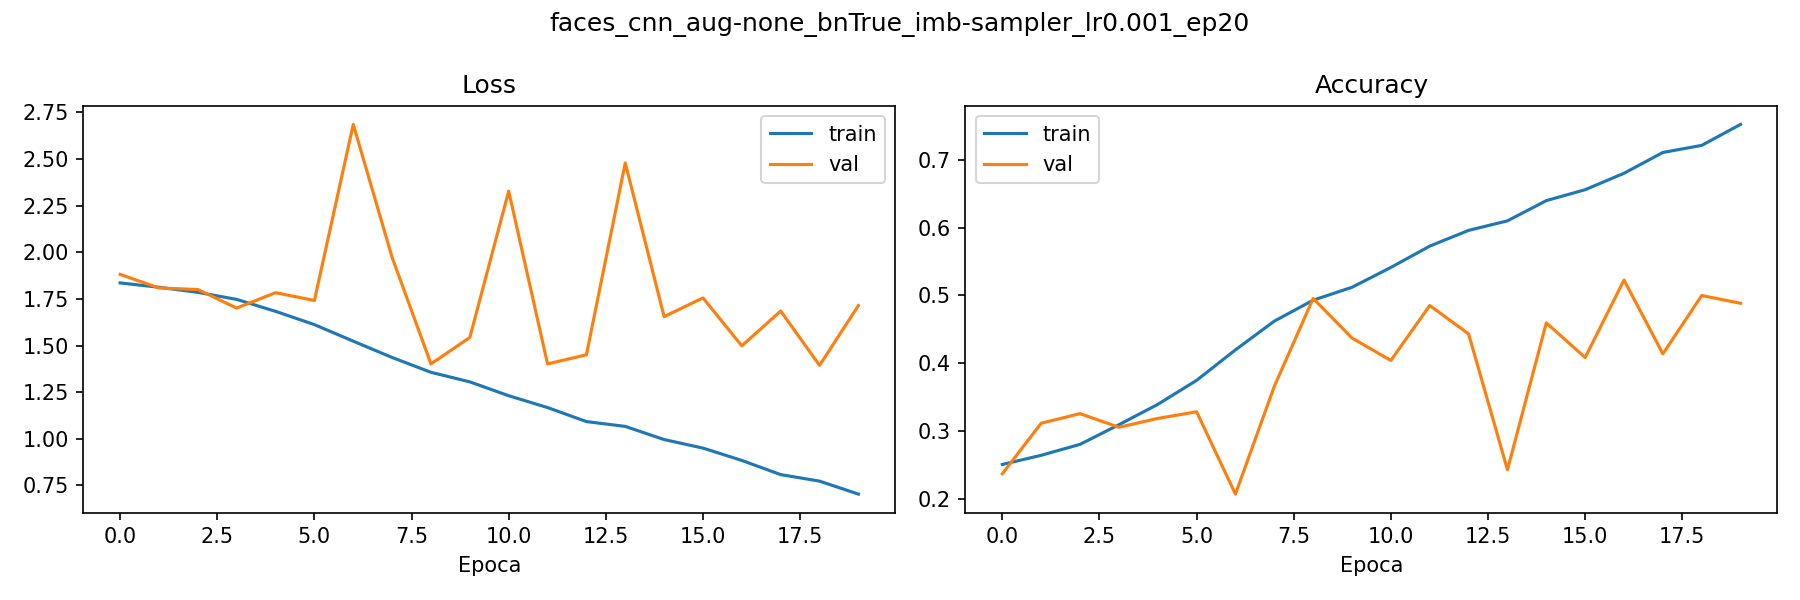
\includegraphics[width=0.48\textwidth]{graphs/imbalance_ablation/faces_sampler_history.png}
\hfill
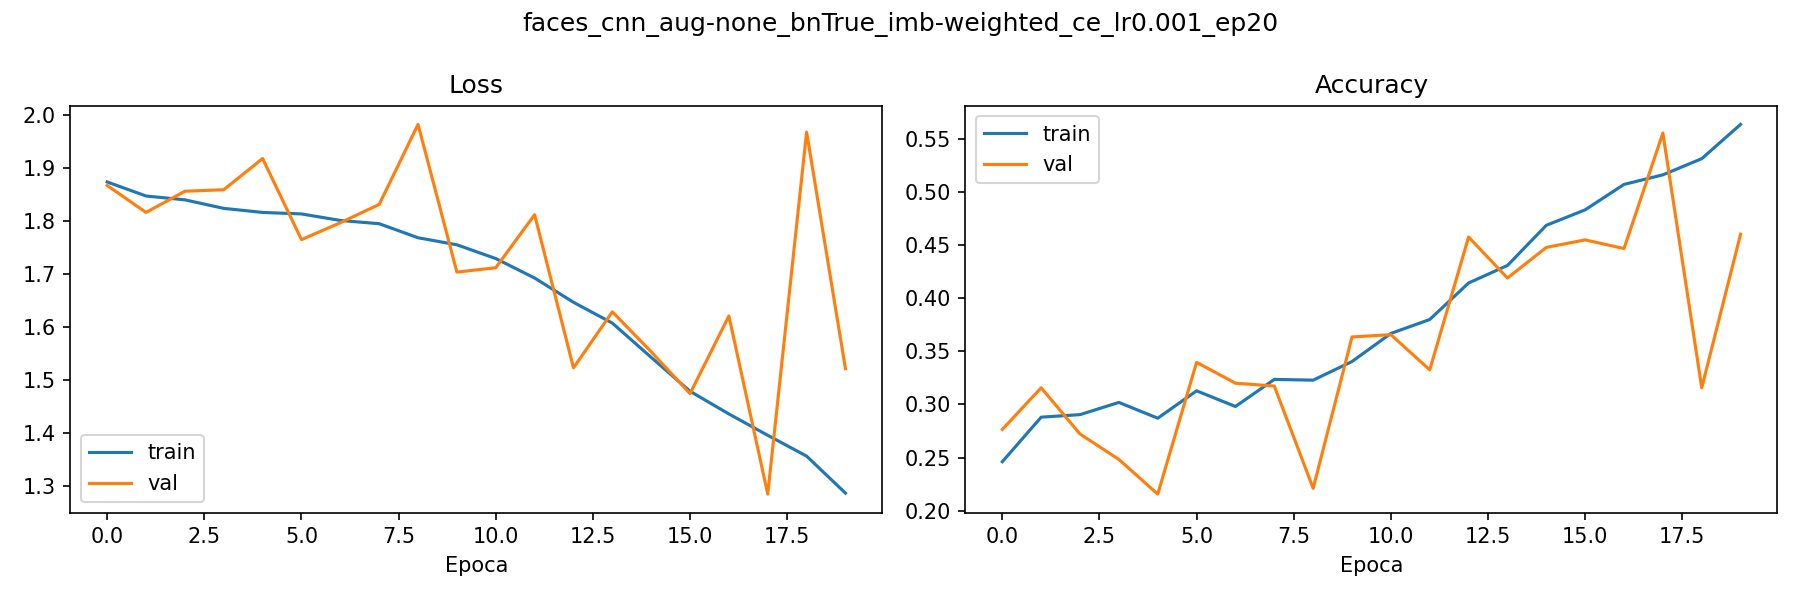
\includegraphics[width=0.48\textwidth]{graphs/imbalance_ablation/faces_weighted_ce_history.png}
\caption{Istoricul antrenării pe Faces cu tehnici de echilibrare: Weighted Random Sampler (stânga) și Weighted Cross Entropy (dreapta)}
\end{figure}

\subsection{Sumar General al Rezultatelor pe Dezechilibru de Clase}
Următorul tabel centralizează comparativ performanțele tehnicilor de rebalansare:
\begin{table}[h!]
\centering
\begin{tabular}{llcl}
\toprule
\textbf{Dataset} & \textbf{Strategie} & \textbf{F1-macro} & \textbf{Obs. cheie} \\
\midrule
Moles & none (baseline) & 0.4624 & \texttt{df} recall=0\% \\
Moles & weighted\_ce & 0.4194 & \texttt{mel} 69\%, \texttt{vasc} 90\%, acc$\downarrow$ \\
Moles & sampler & \textbf{0.4975} & Cel mai bun F1-macro, \texttt{df} reactivat \\
Moles & focal & 0.3628 & Instabil, acuratețe $44\%$ \\
\midrule
Faces & none (baseline) & 0.4229 & \texttt{Fear}/\texttt{Disgust} recall $\sim$0\% \\
Faces & weighted\_ce & 0.4004 & Crește recall-ul \texttt{Fear} la 26\% \\
Faces & sampler & \textbf{0.4740} & Cel mai bun F1-macro, recall \texttt{Fear} 43\% \\
Faces & focal & 0.3028 & Performanță scăzută în 20 epoci \\
\bottomrule
\end{tabular}
\caption{Sumarul performanțelor tehnicilor de echilibrare pe ambele dataset-uri}
\end{table}

\section{Fine-tuning și Transfer Learning cu ResNet-18}
S-a evaluat utilizarea rețelei pre-antrenate \texttt{ResNet-18} (pe ImageNet) în două scenarii distincte de antrenare:
\begin{itemize}
    \item \textbf{Scenariul 1: Backbone înghețat (30 epoci):} S-a antrenat doar clasificatorul liniar final (\texttt{fc}), cu rată de învățare $1e-3$ și augmentări geometrice (cu/fără warmup de 5 epoci).
    \item \textbf{Scenariul 2: Dezghețare selectivă (50 de epoci):} S-au dezghețat ultimele 2 blocuri reziduale (\texttt{layer3} și \texttt{layer4}). S-a utilizat \texttt{WeightedRandomSampler} pentru echilibrarea claselor și augmentări specifice fiecărui set. S-a comparat impactul prezenței/absenței warmup-ului.
\end{itemize}

\subsection{Rezultate și Analiză}
\begin{table}[h!]
\centering
\setlength{\tabcolsep}{4pt}
\makebox[\textwidth][c]{
\begin{tabular}{llcccc}
\toprule
\textbf{Dataset} & \textbf{Configurație ResNet-18} & \textbf{Epoci} & \textbf{Warmup} & \textbf{Acc / F1-micro} & \textbf{F1-macro} \\
\midrule
Moles & Scenariul 1 (Backbone frozen) & 30 & Nu & 0.7489 & 0.5195 \\
Moles & Scenariul 1 (Backbone frozen) & 30 & Da & 0.7404 & 0.4992 \\
Moles & Scenariul 2 (Dezghețat 2 blocuri + Sampler) & 50 & Nu & \textbf{0.8432} & \textbf{0.7267} \\
Moles & Scenariul 2 (Dezghețat 2 blocuri + Sampler) & 50 & Da & 0.8397 & 0.7266 \\
\midrule
Faces & Scenariul 1 (Backbone frozen) & 30 & Nu & 0.5079 & 0.4004 \\
Faces & Scenariul 1 (Backbone frozen) & 30 & Da & 0.5231 & 0.3971 \\
Faces & Scenariul 2 (Dezghețat 2 blocuri + Sampler) & 50 & Nu & 0.7703 & 0.6741 \\
Faces & Scenariul 2 (Dezghețat 2 blocuri + Sampler) & 50 & Da & \textbf{0.7790} & \textbf{0.6784} \\
\bottomrule
\end{tabular}
}
\caption{Impactul dezghețării selective și al warmup-ului pe ResNet-18}
\end{table}

\textbf{Analiză unfreezing-ului și a warmup-ului (supra-reglaj / sub-reglaj):}\\
Înghețarea completă a backbone-ului (Scenariul 1) limitează F1-macro la $\sim 0.52$ (Moles) și $\sim 0.40$ (Faces), indicând sub-reglaj din cauza capacității reduse a modelului. Dezghețarea ultimelor 2 blocuri reziduale (Scenariul 2) determină o creștere masivă a F1-macro la \textbf{0.7267} (Moles) și \textbf{0.6784} (Faces), indicând necesitatea adaptării filtrelor convoluționale. Procedura de warmup aduce un beneficiu în Scenariul 2 pe setul \texttt{Faces} ($0.6784$ vs $0.6741$), stabilizând antrenarea în prezența datelor augmentate, efect ilustrat prin curbele comparative din Figura~\ref{fig:faces_resnet18_scenariul2} (iar pentru Scenariul 1 în Figura~\ref{fig:faces_resnet18_scenariul1}).

\begin{figure}[h!]
\centering
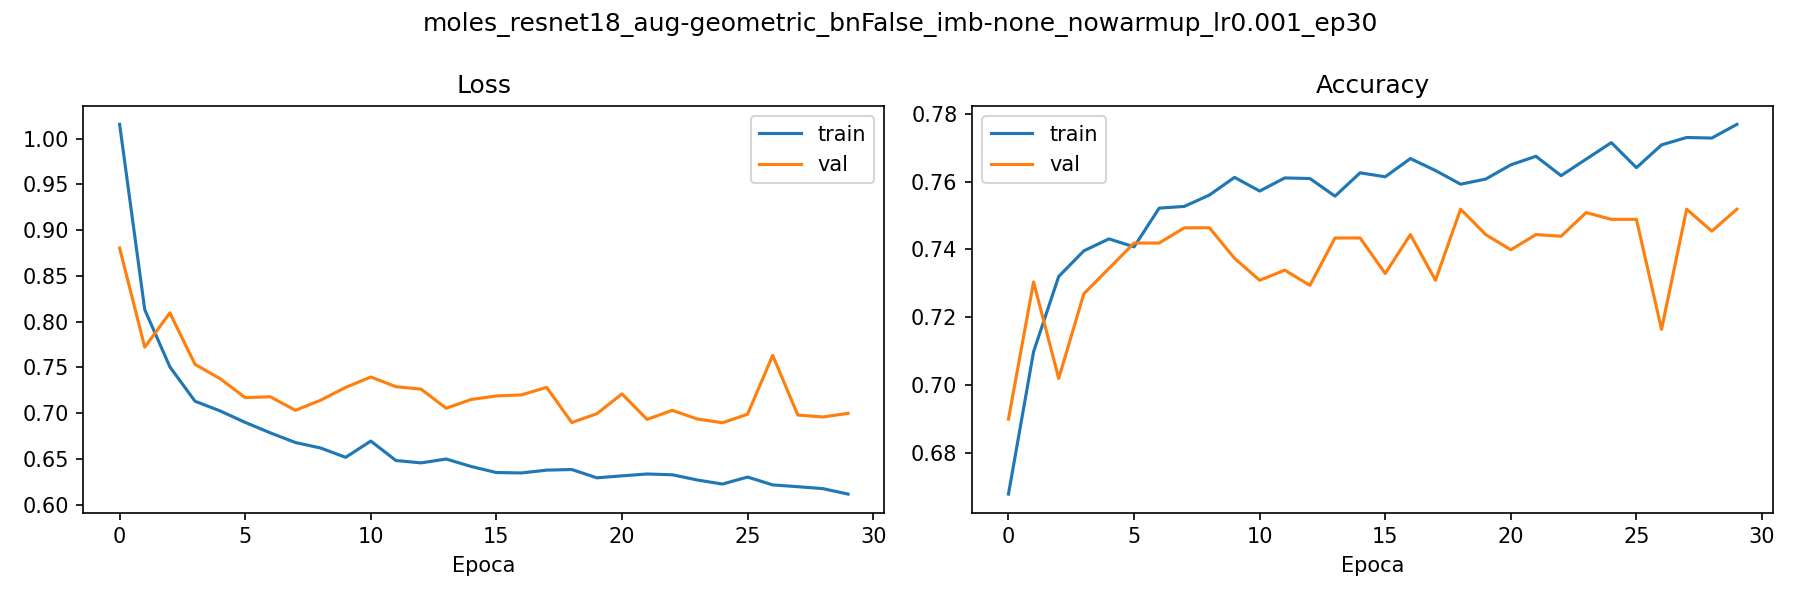
\includegraphics[width=0.48\textwidth]{graphs/moles_resnet18_aug-geometric_bnFalse_imb-none_nowarmup_lr0.001_ep30_history.png}
\hfill
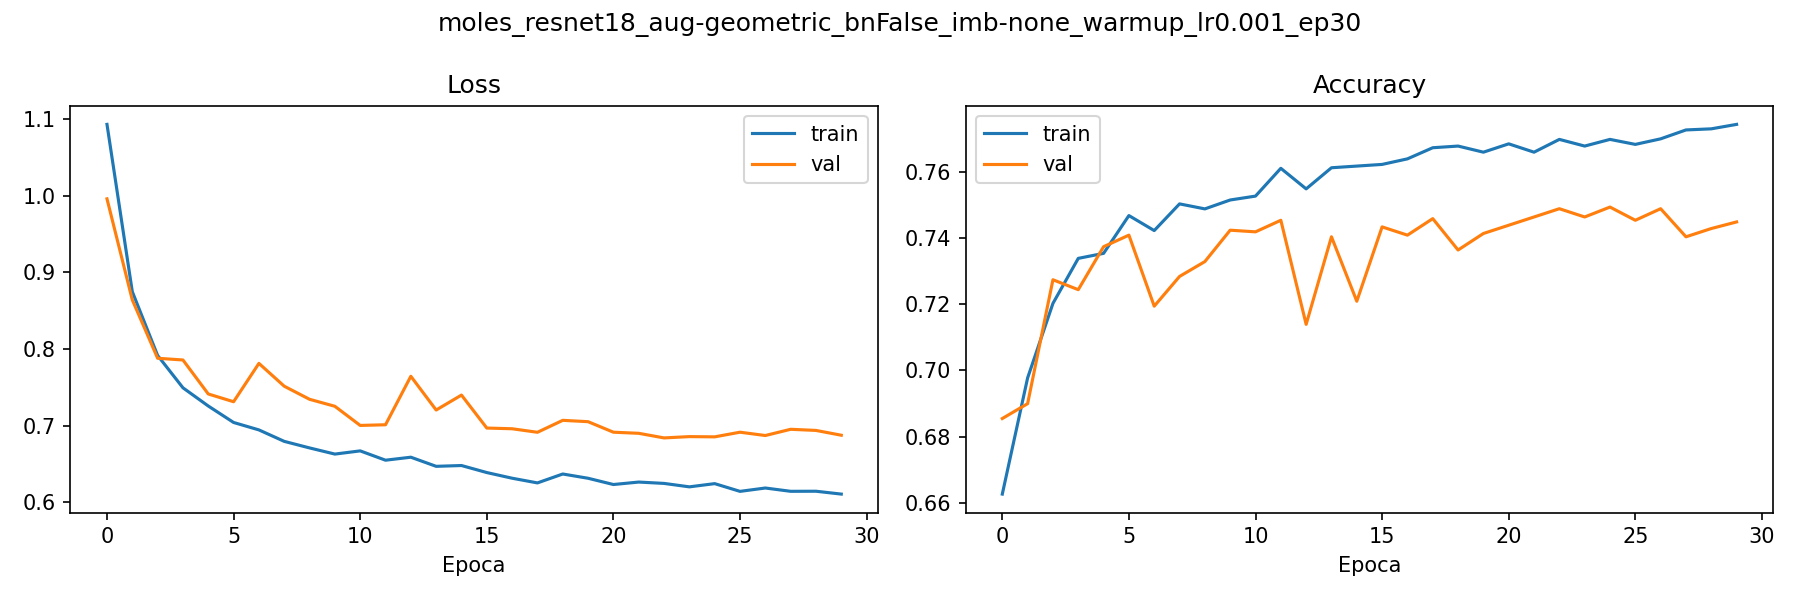
\includegraphics[width=0.48\textwidth]{graphs/moles_resnet18_aug-geometric_bnFalse_imb-none_warmup_lr0.001_ep30_history.png}
\caption{Evoluție ResNet-18 pe Moles în Scenariul 1: Fără Warmup (stânga) vs. Cu Warmup (dreapta)}
\end{figure}

\begin{figure}[h!]
\centering
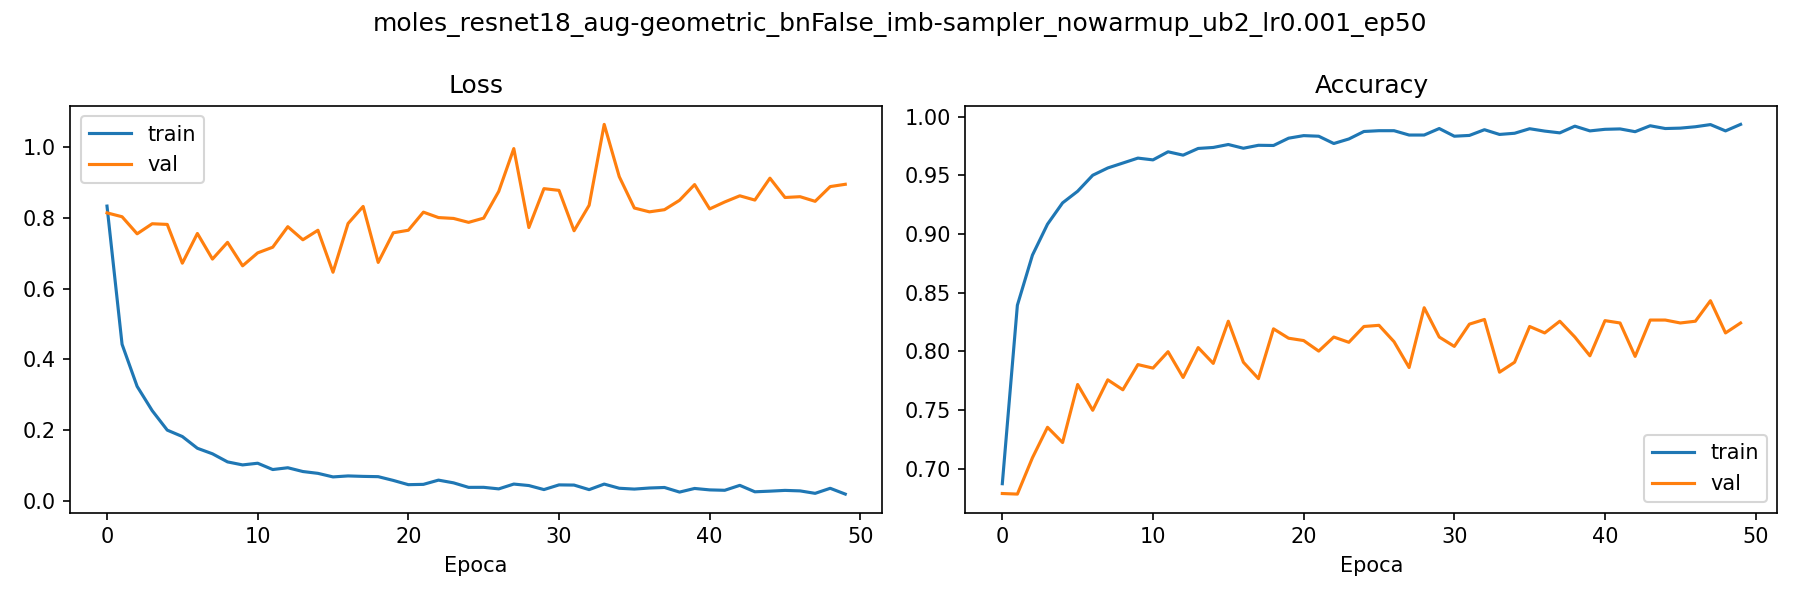
\includegraphics[width=0.48\textwidth]{graphs/moles_resnet18_aug-geometric_bnFalse_imb-sampler_nowarmup_ub2_lr0.001_ep50_history.png}
\hfill
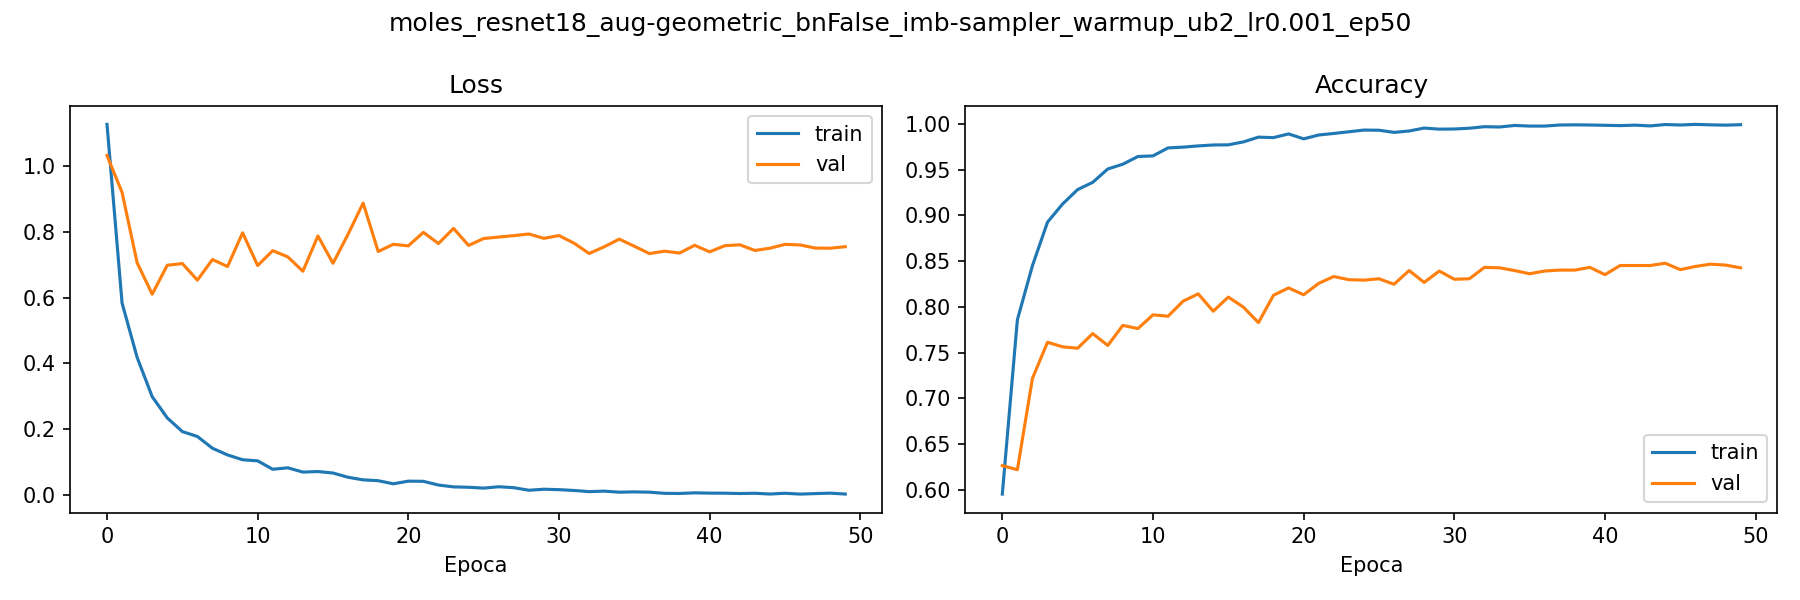
\includegraphics[width=0.48\textwidth]{graphs/moles_resnet18_aug-geometric_bnFalse_imb-sampler_warmup_ub2_lr0.001_ep50_history.png}
\caption{Evoluție ResNet-18 pe Moles în Scenariul 2: Fără Warmup (stânga) vs. Cu Warmup (dreapta)}
\end{figure}

\begin{figure}[h!]
\centering
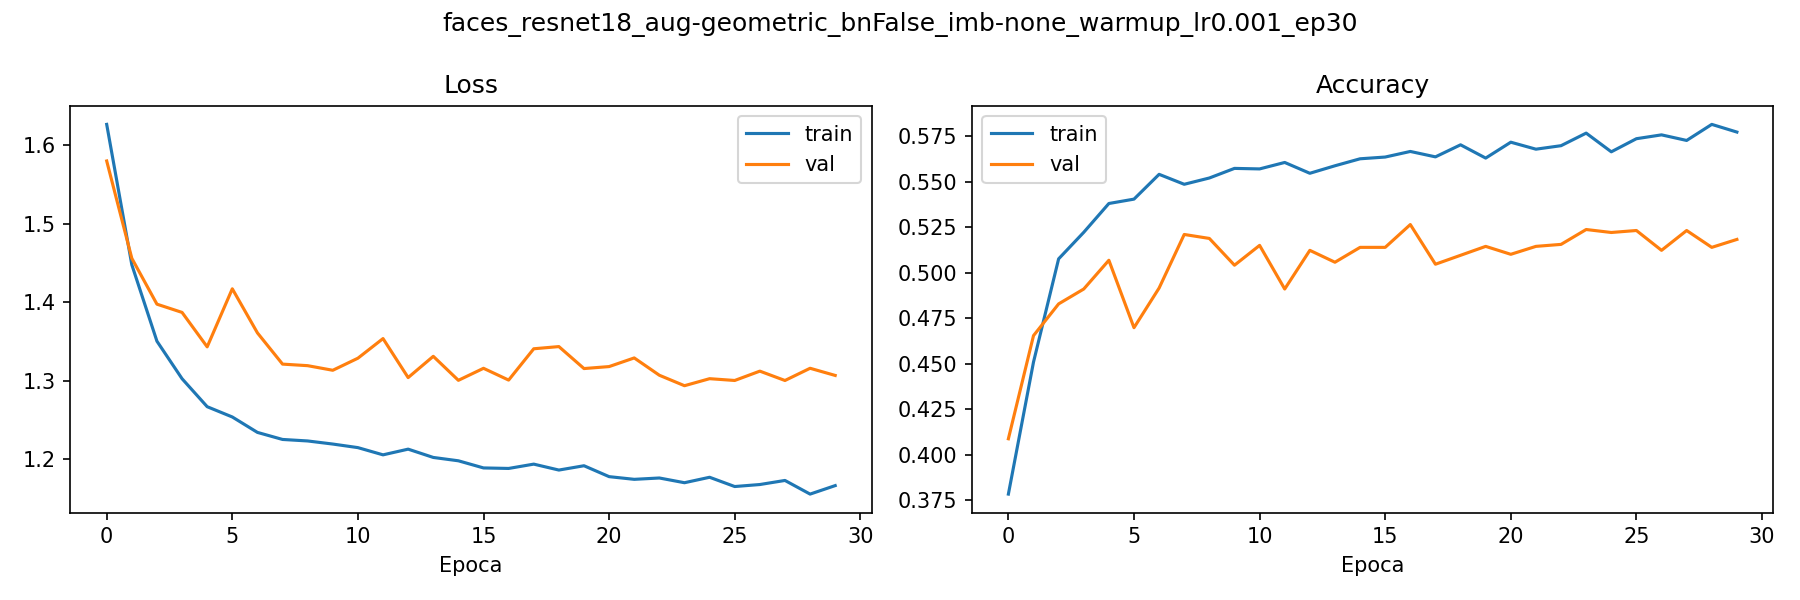
\includegraphics[width=0.6\textwidth]{graphs/faces_resnet18_aug-geometric_bnFalse_imb-none_warmup_lr0.001_ep30_history.png}
\caption{Evoluție ResNet-18 pe Faces în Scenariul 1 (cu Warmup)}
\label{fig:faces_resnet18_scenariul1}
\end{figure}

\begin{figure}[h!]
\centering
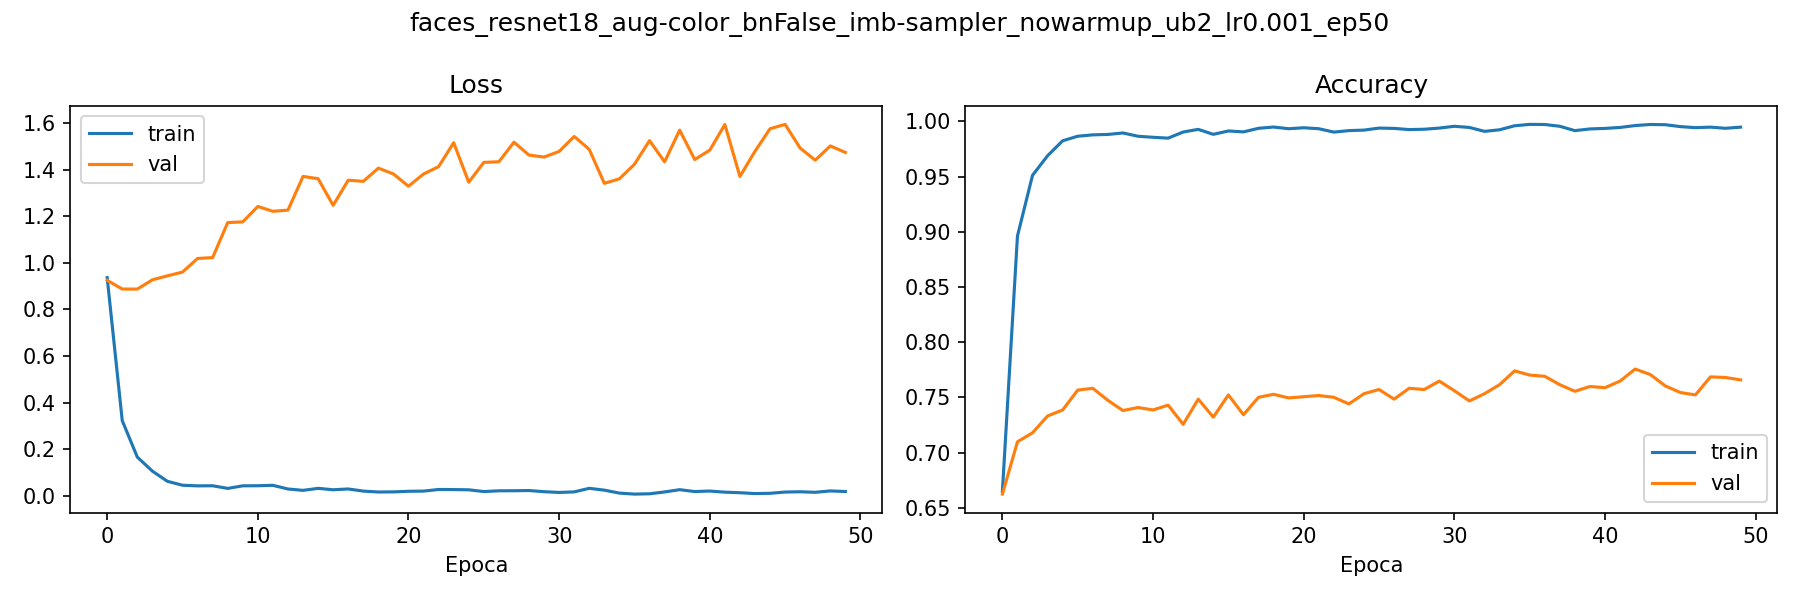
\includegraphics[width=0.48\textwidth]{graphs/faces_resnet18_aug-color_bnFalse_imb-sampler_nowarmup_ub2_lr0.001_ep50_history.png}
\hfill
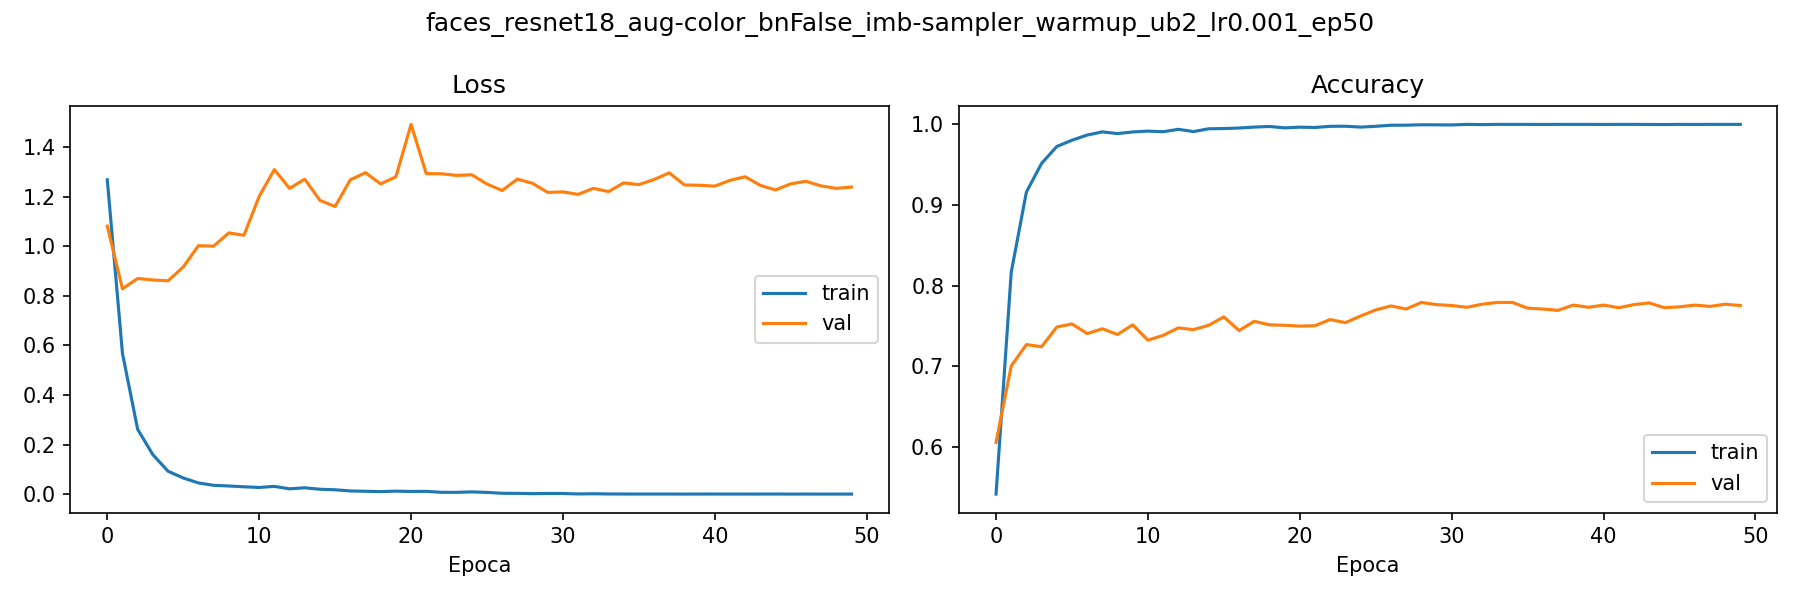
\includegraphics[width=0.48\textwidth]{graphs/faces_resnet18_aug-color_bnFalse_imb-sampler_warmup_ub2_lr0.001_ep50_history.png}
\caption{Evoluție ResNet-18 pe Faces în Scenariul 2: Fără Warmup (stânga) vs. Cu Warmup (dreapta)}
\label{fig:faces_resnet18_scenariul2}
\end{figure}

\section{Curriculum Learning pe setul de date Moles (Bonus 4.1)}
S-a evaluat impactul Curriculum Learning pe setul de date \texttt{Moles}, utilizând modelul \texttt{ResNet-18} pre-antrenat cu ultimele 2 blocuri reziduale dezghețate, antrenat timp de 40 de epoci cu ponderea claselor (Weighted CE) și scheduler \texttt{CosineAnnealing}.

\subsection{Definirea Dificultății și Funcția de Pacing}
\begin{enumerate}
    \item \textbf{Definirea dificultății imaginii:} Ca proxy pentru dificultate, s-a utilizat:
    \[
    \text{Dificultate} = 1.0 - \text{Var}_{\text{norm}}(\text{imagine})
    \]
    unde varianța normalizată reprezintă contrastul imaginii grayscale. Distribuția scorurilor calculate este prezentată în Figura~\ref{fig:cl_difficulty} (stânga).
    
    \item \textbf{Funcția de pacing (Strategia 1):} La epoca 0 se începe cu primele 30\% cele mai ușoare imagini, crescând proporția liniar până la 100\% la epoca 20, valoare menținută constantă ulterior (Figura~\ref{fig:cl_difficulty}, dreapta).
    
    \item \textbf{Self-Paced Learning (Strategia 2):} La fiecare epocă se calculează funcția de cost a modelului pe fiecare imagine. Sunt reținute pentru antrenare doar imaginile cu o valoare a funcției de cost mai mică decât percentila curentă $q$, unde $q$ crește liniar de la $0.3$ la $1.0$ (cu un pas de $0.05$ pe epocă).
\end{enumerate}

\begin{figure}[h!]
\centering
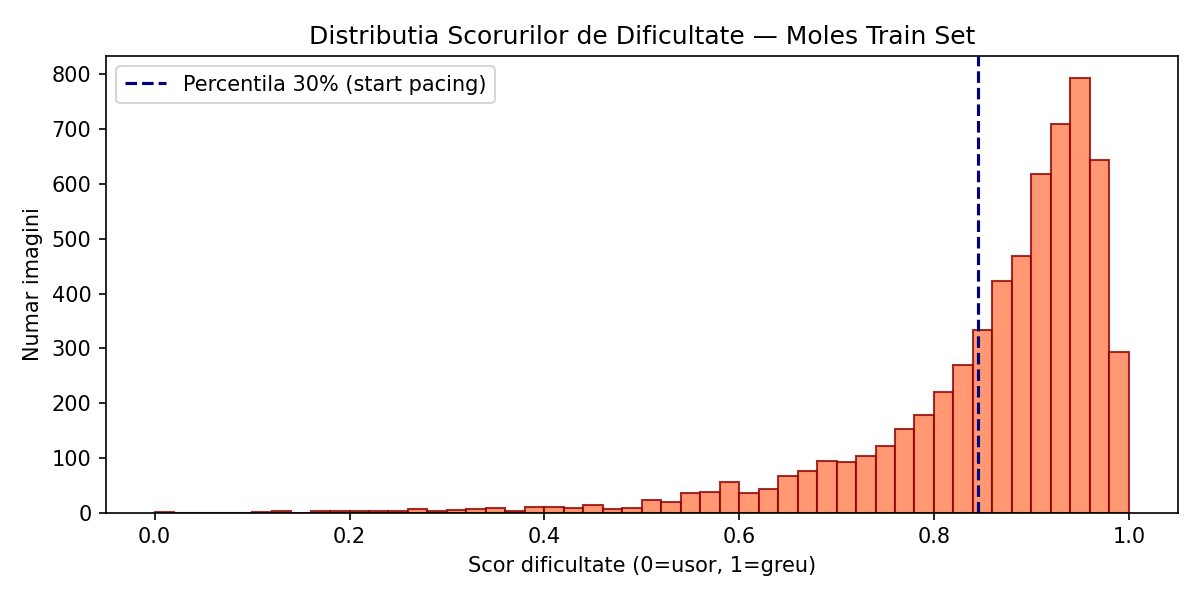
\includegraphics[width=0.48\textwidth]{graphs/moles_cl_difficulty_distribution.png}
\hfill
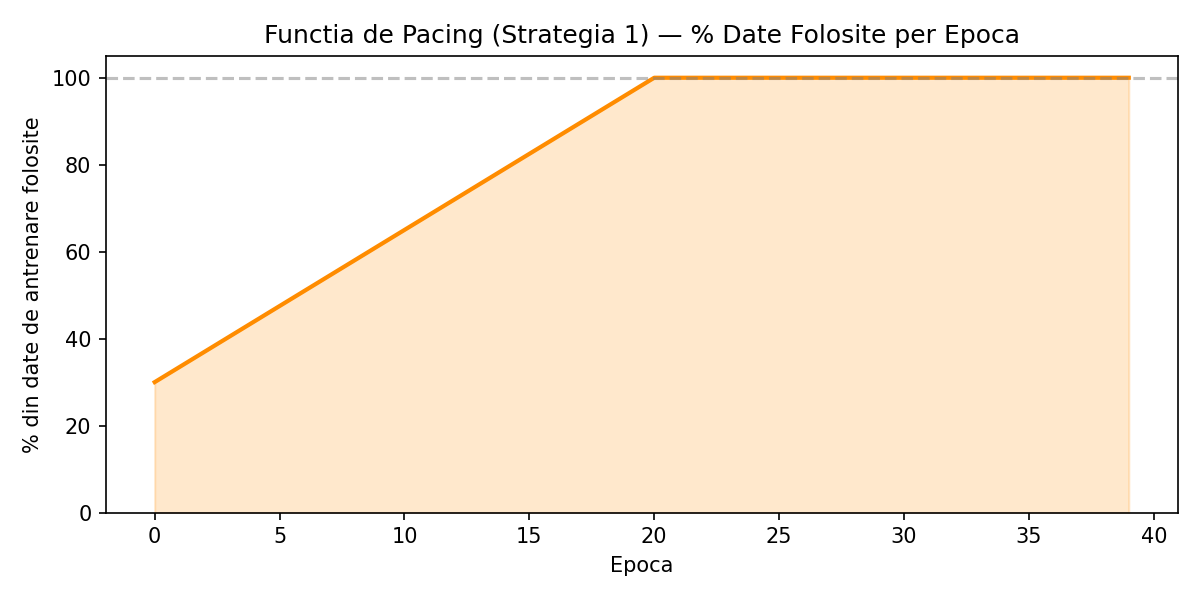
\includegraphics[width=0.48\textwidth]{graphs/moles_cl_pacing_curve.png}
\caption{Distribuția dificultății pe setul Moles (stânga) și funcția de pacing static (dreapta)}
\label{fig:cl_difficulty}
\end{figure}

\subsection{Rezultate și Analiză Comparativă}
S-au comparat performanțele pe setul de validare locală pentru cele trei scenarii antrenate timp de 40 de epoci:

\begin{table}[h!]
\centering
\begin{tabular}{lcc}
\toprule
\textbf{Strategie Antrenare} & \textbf{Val Acc / F1-Micro} & \textbf{F1-Macro Val} \\
\midrule
Baseline (fără CL) & 82.68\% & \textbf{0.7489} \\
Strategia 1 (Pacing Static) & \textbf{83.13\%} & 0.7277 \\
Strategia 2 (Self-Paced) & 82.73\% & 0.7228 \\
\bottomrule
\end{tabular}
\caption{Comparație Curriculum Learning pe setul Moles}
\label{tab:cl_results}
\end{table}

\begin{figure}[h!]
\centering
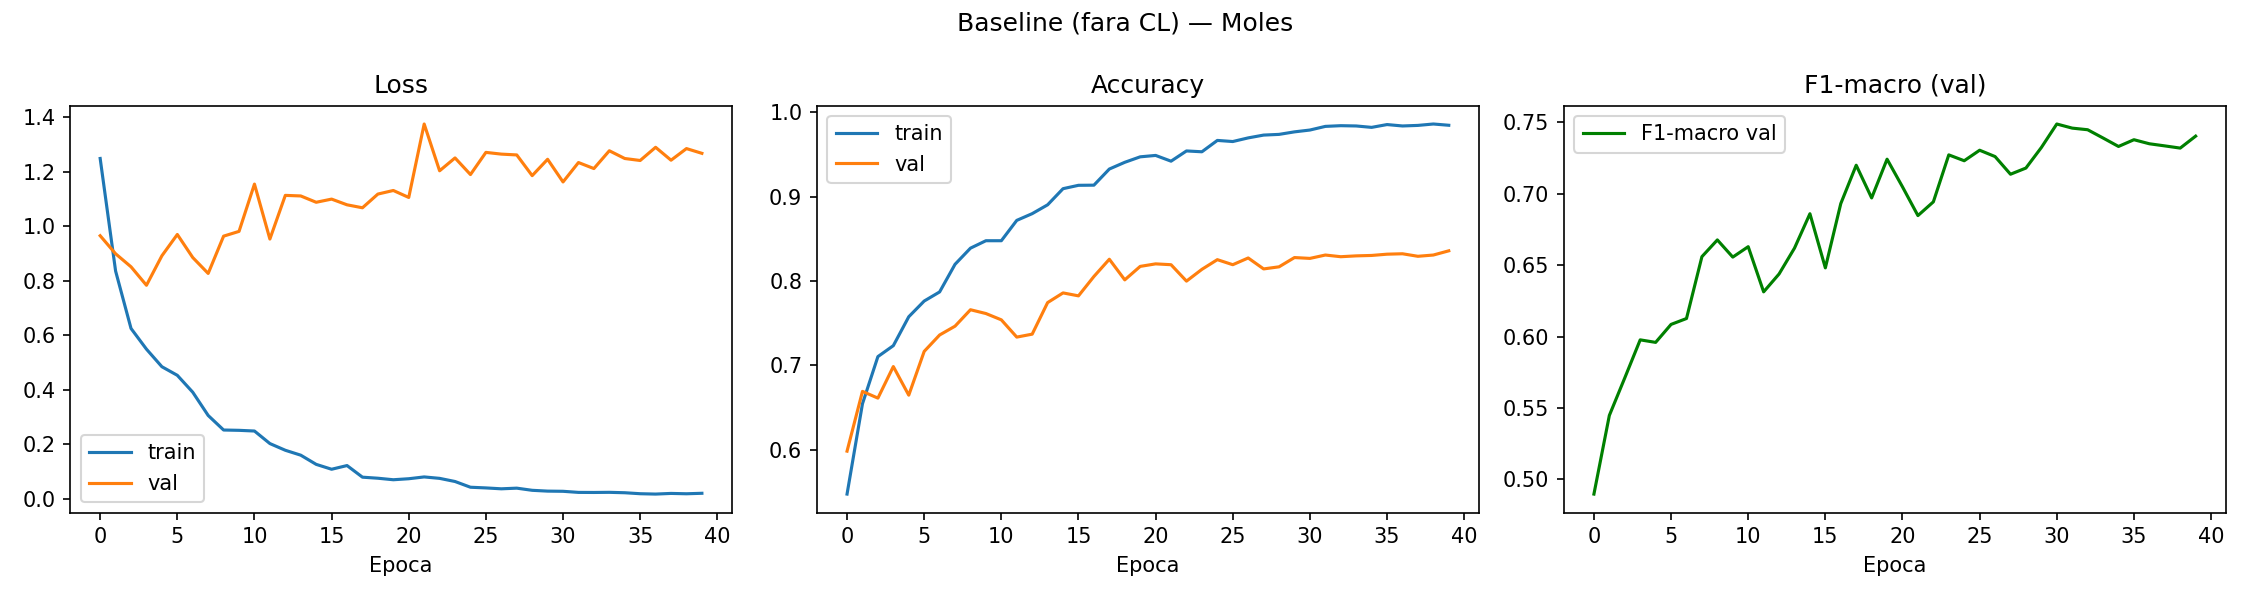
\includegraphics[width=0.75\textwidth]{graphs/moles_cl_baseline_history.png}
\\ \vspace{0.2cm}
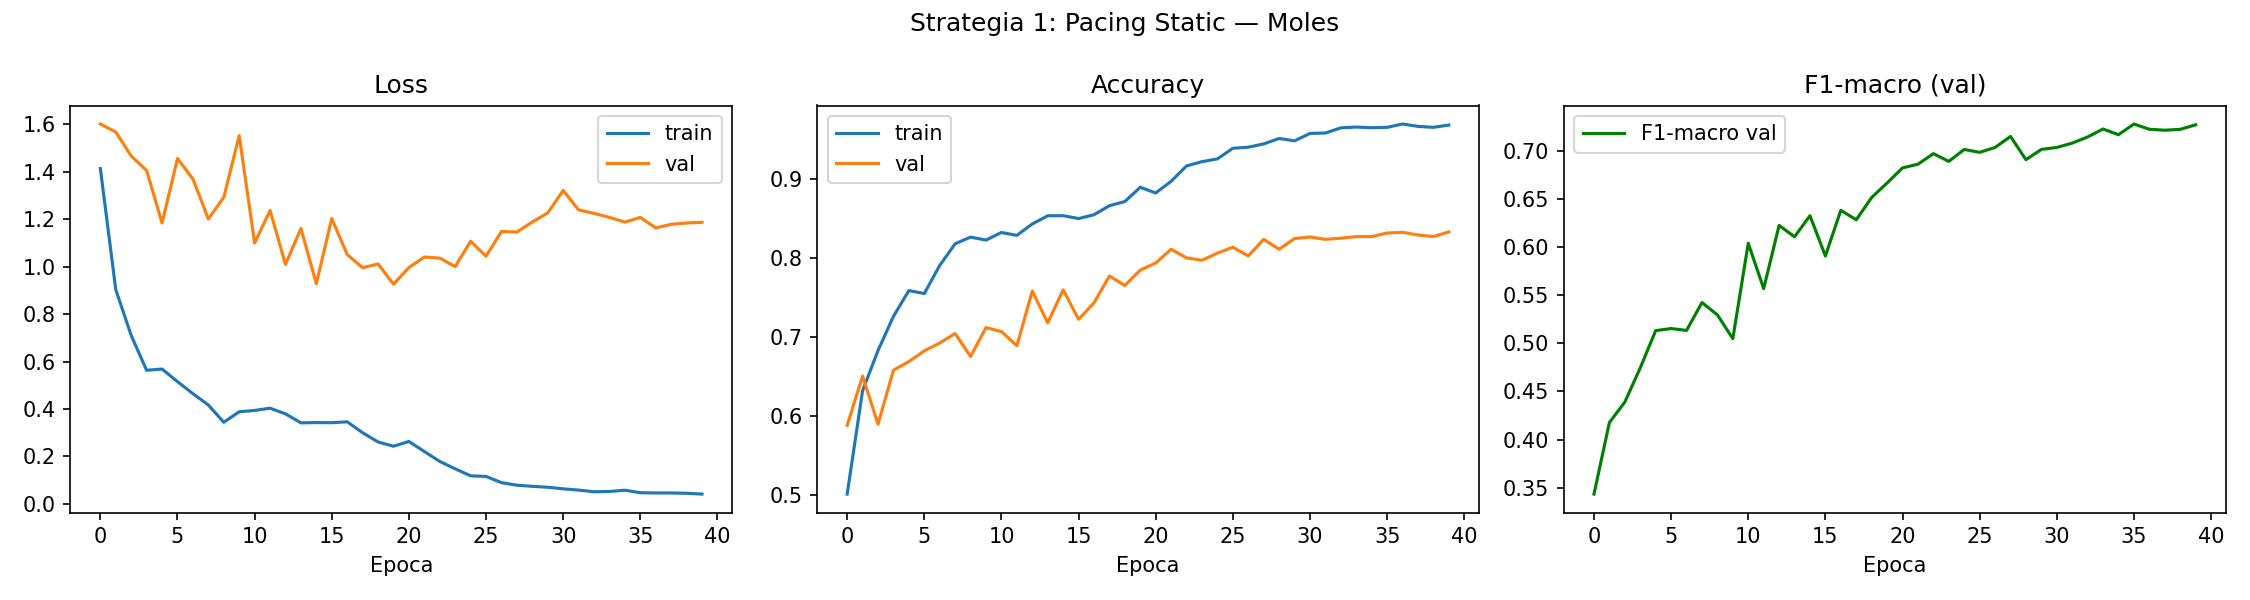
\includegraphics[width=0.75\textwidth]{graphs/moles_cl_strategy1_history.png}
\caption{Istoricul antrenării pe Moles: Baseline (sus) vs. Strategia 1 Pacing Static (jos)}
\end{figure}

\begin{figure}[h!]
\centering
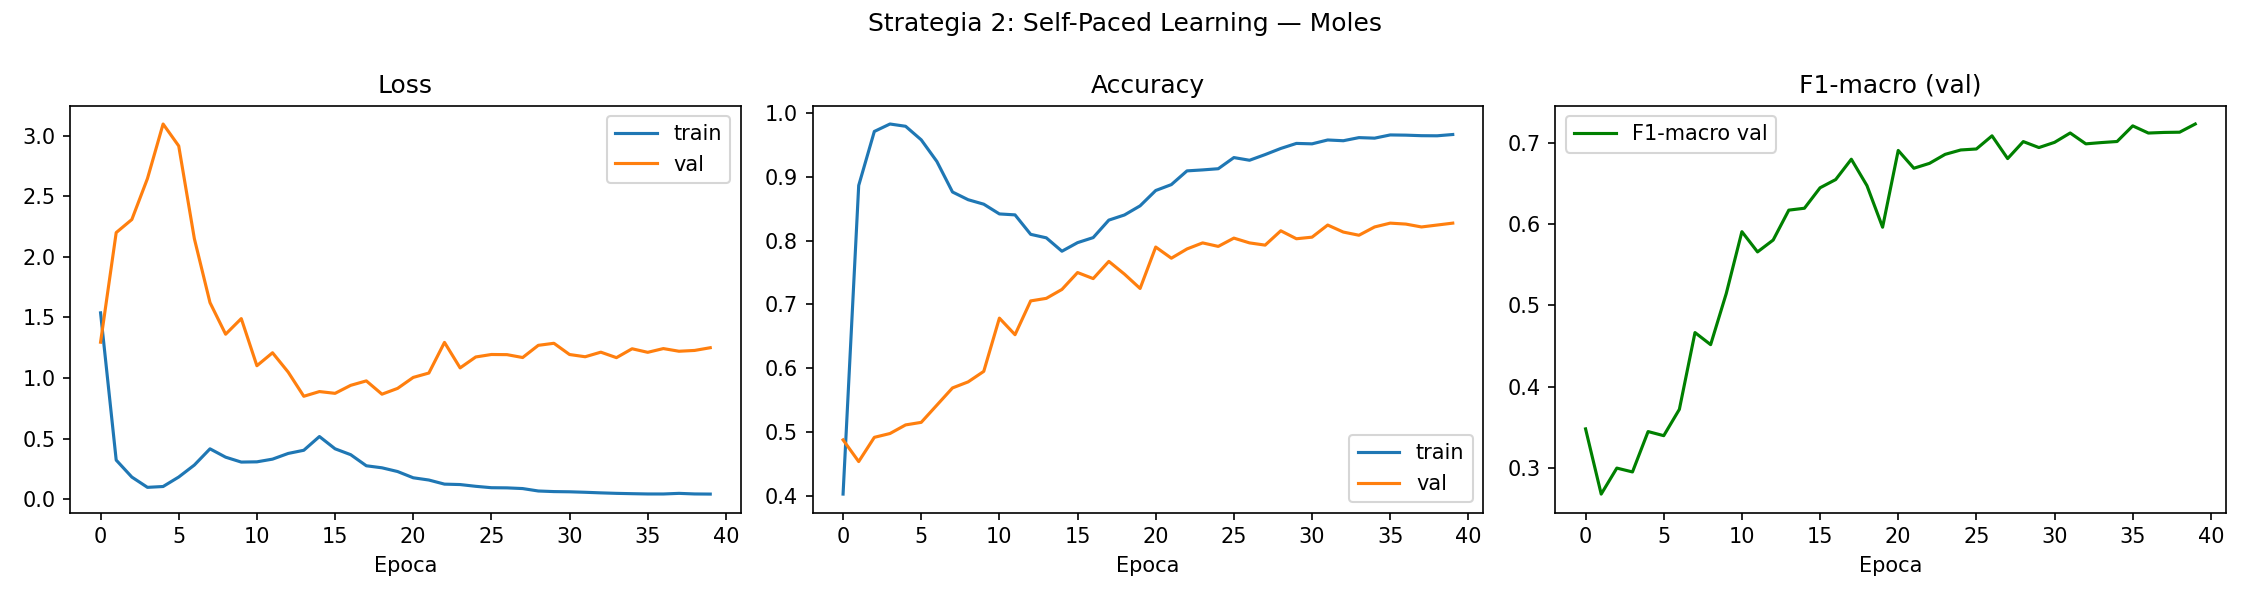
\includegraphics[width=0.75\textwidth]{graphs/moles_cl_strategy2_history.png}
\\ \vspace{0.2cm}
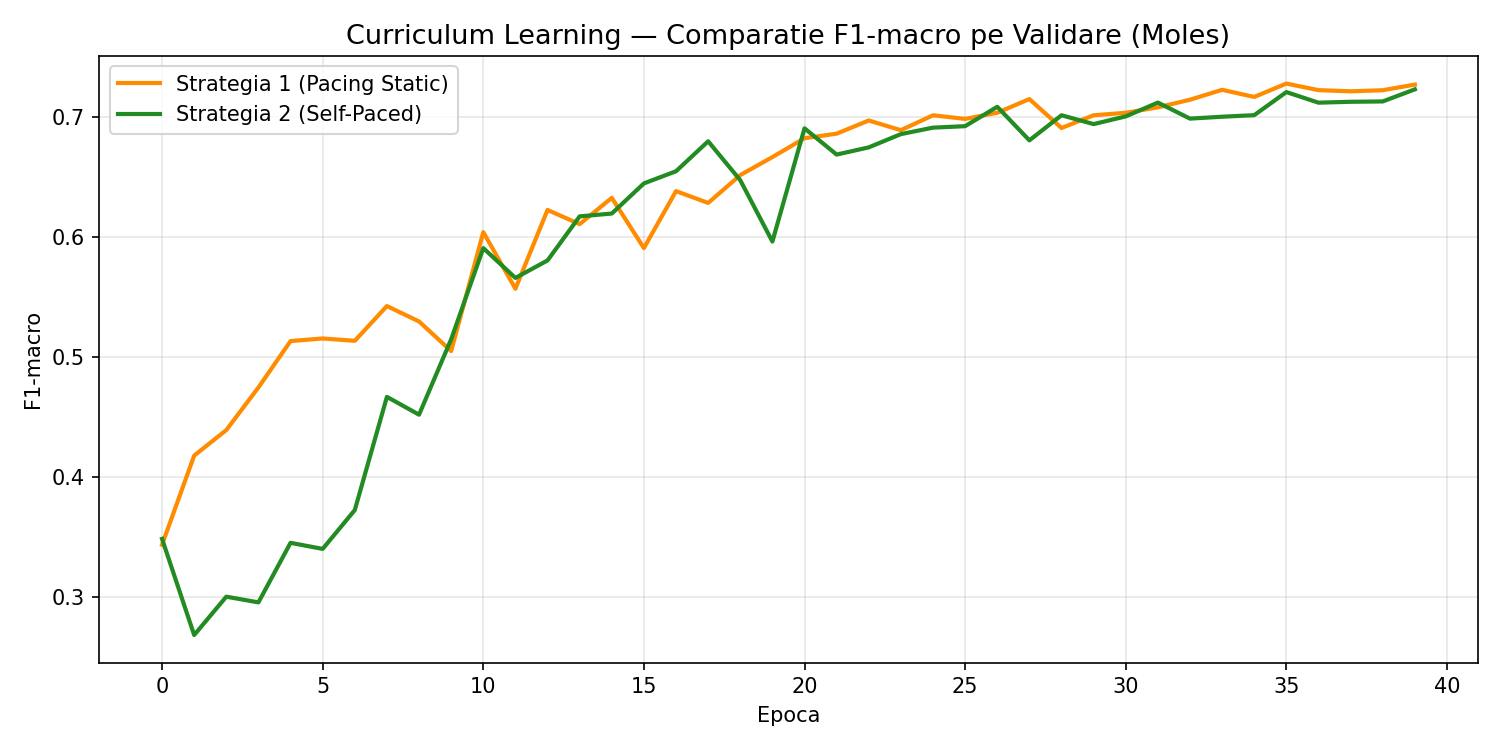
\includegraphics[width=0.75\textwidth]{graphs/moles_cl_comparison.png}
\caption{Istoricul antrenării pentru Strategia 2 Self-Paced (sus) și curbele F1-macro comparate pe validare (jos)}
\label{fig:cl_curves}
\end{figure}

\subsection{Concluzii Studiu Curriculum Learning}
Analiza curbelor și a metricilor relevă următoarele aspecte:
\begin{itemize}
    \item \textbf{Impactul dezechilibrului:} Pacing-ul static (Strategia 1) a crescut acuratețea globală la $83.13\%$, dar a redus F1-macro la $0.7277$ (de la $0.7489$). Acest lucru se datorează faptului că imaginile din clasa majoritară \texttt{nv} au un contrast mai mare (fiind considerate „ușoare”) și domină batch-urile inițiale, privând modelul de contactul timpuriu cu clasele rare.
    \item \textbf{Limitarea Self-Paced:} Strategia 2 a redus F1-macro la $0.7228$. Selectarea dinamică a mostrelor cu cost mic a favorizat exclusiv clasa majoritară \texttt{nv}, împiedicând învățarea claselor rare în primele epoci.
\end{itemize}
Astfel, curriculum learning pe seturi dezechilibrate necesită eșantionare stratificată pentru a preveni dominanța clasei majoritare.

\section{Modele Finale, Ensemble și Tehnica TTA}
Pentru maximizarea performanței pe setul \texttt{Faces}, s-a antrenat arhitectura \texttt{ResNet-18} timp de 120 de epoci utilizând:
\begin{itemize}
    \item Dezghețarea tuturor celor 4 blocuri reziduale (\texttt{layer1}–\texttt{layer4}).
    \item Cap de clasificare complex: \texttt{Linear(512)} $\rightarrow$ \texttt{BatchNorm1d} $\rightarrow$ \texttt{ReLU} $\rightarrow$ \texttt{Dropout(0.3)} $\rightarrow$ \texttt{Linear(256} $\rightarrow$ \texttt{7)}.
    \item Rate de învățare diferențiate: $1e-4$ pe backbone și $1e-3$ pe clasificator, cu scheduler \texttt{CosineAnnealingLR}.
    \item Augmentări complete (\texttt{all}) și antrenare cu trei inițializări (seeds) diferite.
\end{itemize}

\subsection{Configurația Finală și Rulările Multi-Seed}
\begin{table}[h!]
\centering
\begin{tabular}{llccc}
\toprule
\textbf{Dataset} & \textbf{Model Rulat (120 epoci)} & \textbf{Val Acc / F1-Micro} & \textbf{F1-Macro Val} \\
\midrule
Faces & Rulare Standard & 82.04\% & \textbf{0.7408} \\
Faces & Rulare Seed 42 & 82.04\% & 0.7382 \\
Faces & Rulare Seed 123 & \textbf{82.47\%} & 0.7298 \\
\bottomrule
\end{tabular}
\caption{Performanțele modelelor finale de 120 de epoci pe setul Faces}
\end{table}

\begin{figure}[h!]
\centering
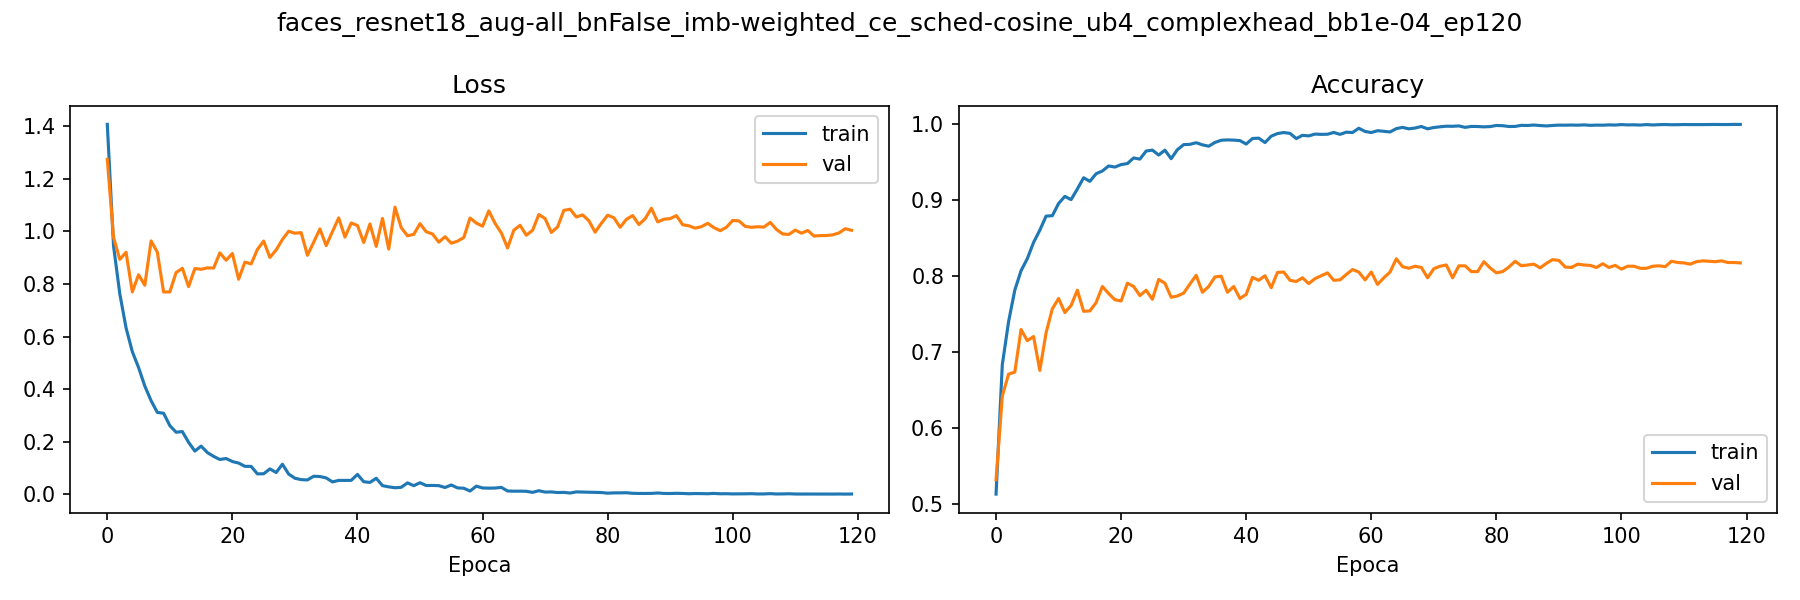
\includegraphics[width=0.48\textwidth]{graphs/faces_resnet18_aug-all_bnFalse_imb-weighted_ce_sched-cosine_ub4_complexhead_bb1e-04_ep120_history.png}
\hfill
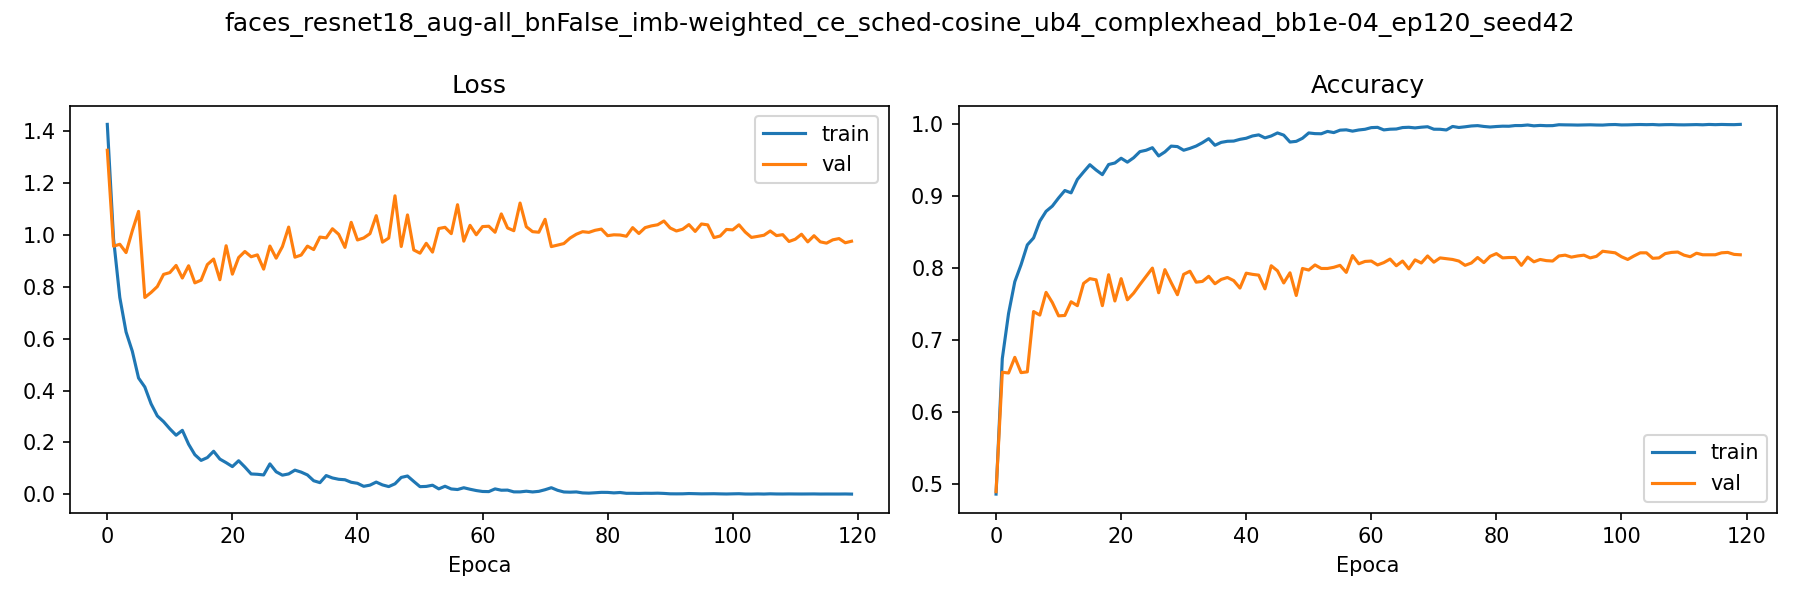
\includegraphics[width=0.48\textwidth]{graphs/faces_resnet18_aug-all_bnFalse_imb-weighted_ce_sched-cosine_ub4_complexhead_bb1e-04_ep120_seed42_history.png}
\caption{Evoluție antrenare Faces: Rularea Standard (stânga) și Seed 42 (dreapta)}
\end{figure}

\begin{figure}[h!]
\centering
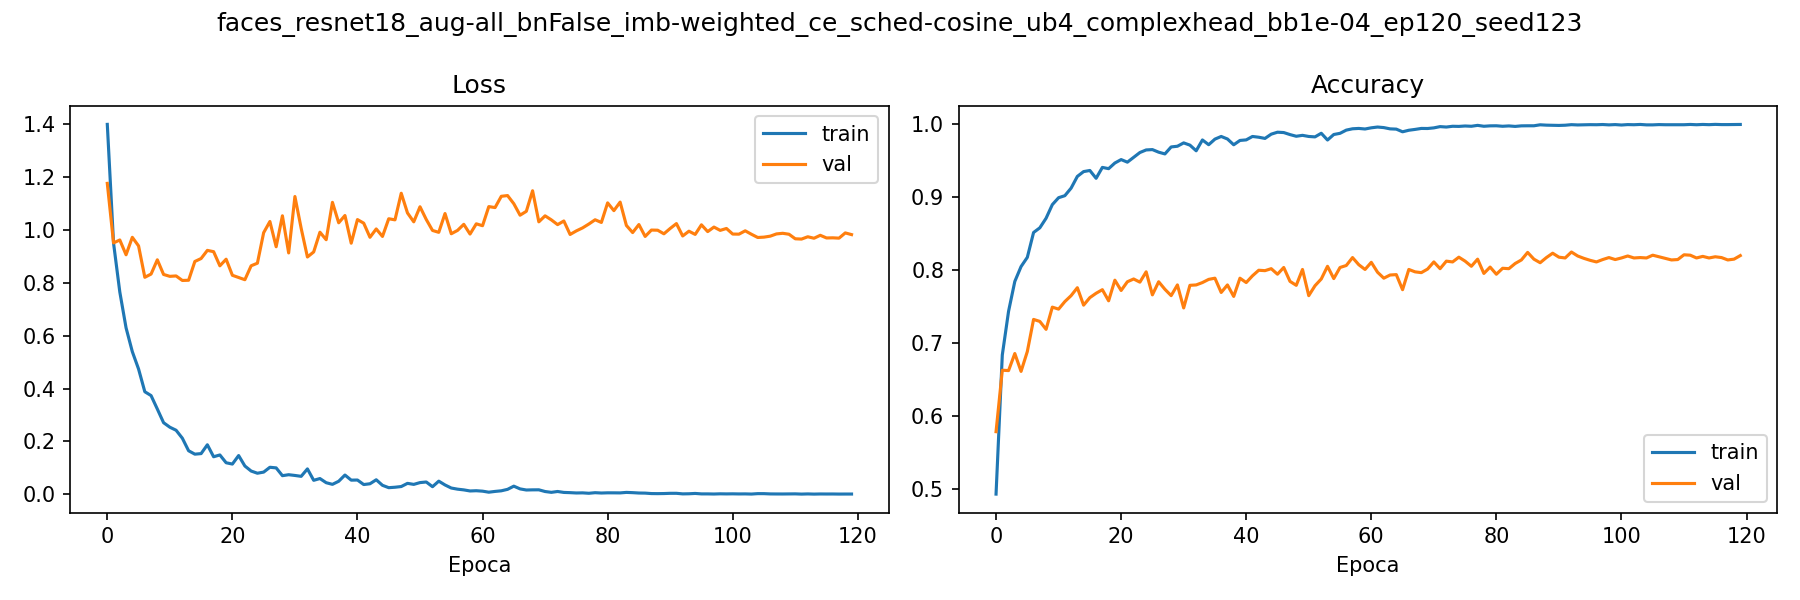
\includegraphics[width=0.6\textwidth]{graphs/faces_resnet18_aug-all_bnFalse_imb-weighted_ce_sched-cosine_ub4_complexhead_bb1e-04_ep120_seed123_history.png}
\caption{Evoluție antrenare Faces: Rularea Seed 123}
\end{figure}

\subsection{Test-Time Augmentation (TTA)}
La inferență, s-a aplicat Test-Time Augmentation prin medierea logiților imaginii originale și ai versiunii sale reflectate orizontal (horizontal flip). Această tehnică reduce variabilitatea predicțiilor și îmbunătățește scorul F1-macro.

\subsection{Medierea Logiților (Ensemble)}
Pentru reducerea varianței, s-a realizat un ansamblu (ensemble) prin medierea aritmetică a logiților celor trei modele antrenate (Standard, Seed 42, Seed 123):
\[
\text{Logits}_{\text{Ensemble}} = \frac{\text{Logits}_{\text{Standard}} + \text{Logits}_{\text{Seed42}} + \text{Logits}_{\text{Seed123}}}{3}
\]
Această mediere a condus la o decizie stabilă și a permis depășirea pragului de performanță stabilit.

\subsection{Matrice de Confuzie și Metrici Finale}
Pentru ilustrarea performanței pe fiecare clasă, se prezintă matricele de confuzie obținute pe seturile de validare locală pentru cele mai bune configurații de pe ambele seturi de date:

\begin{figure}[h!]
\centering
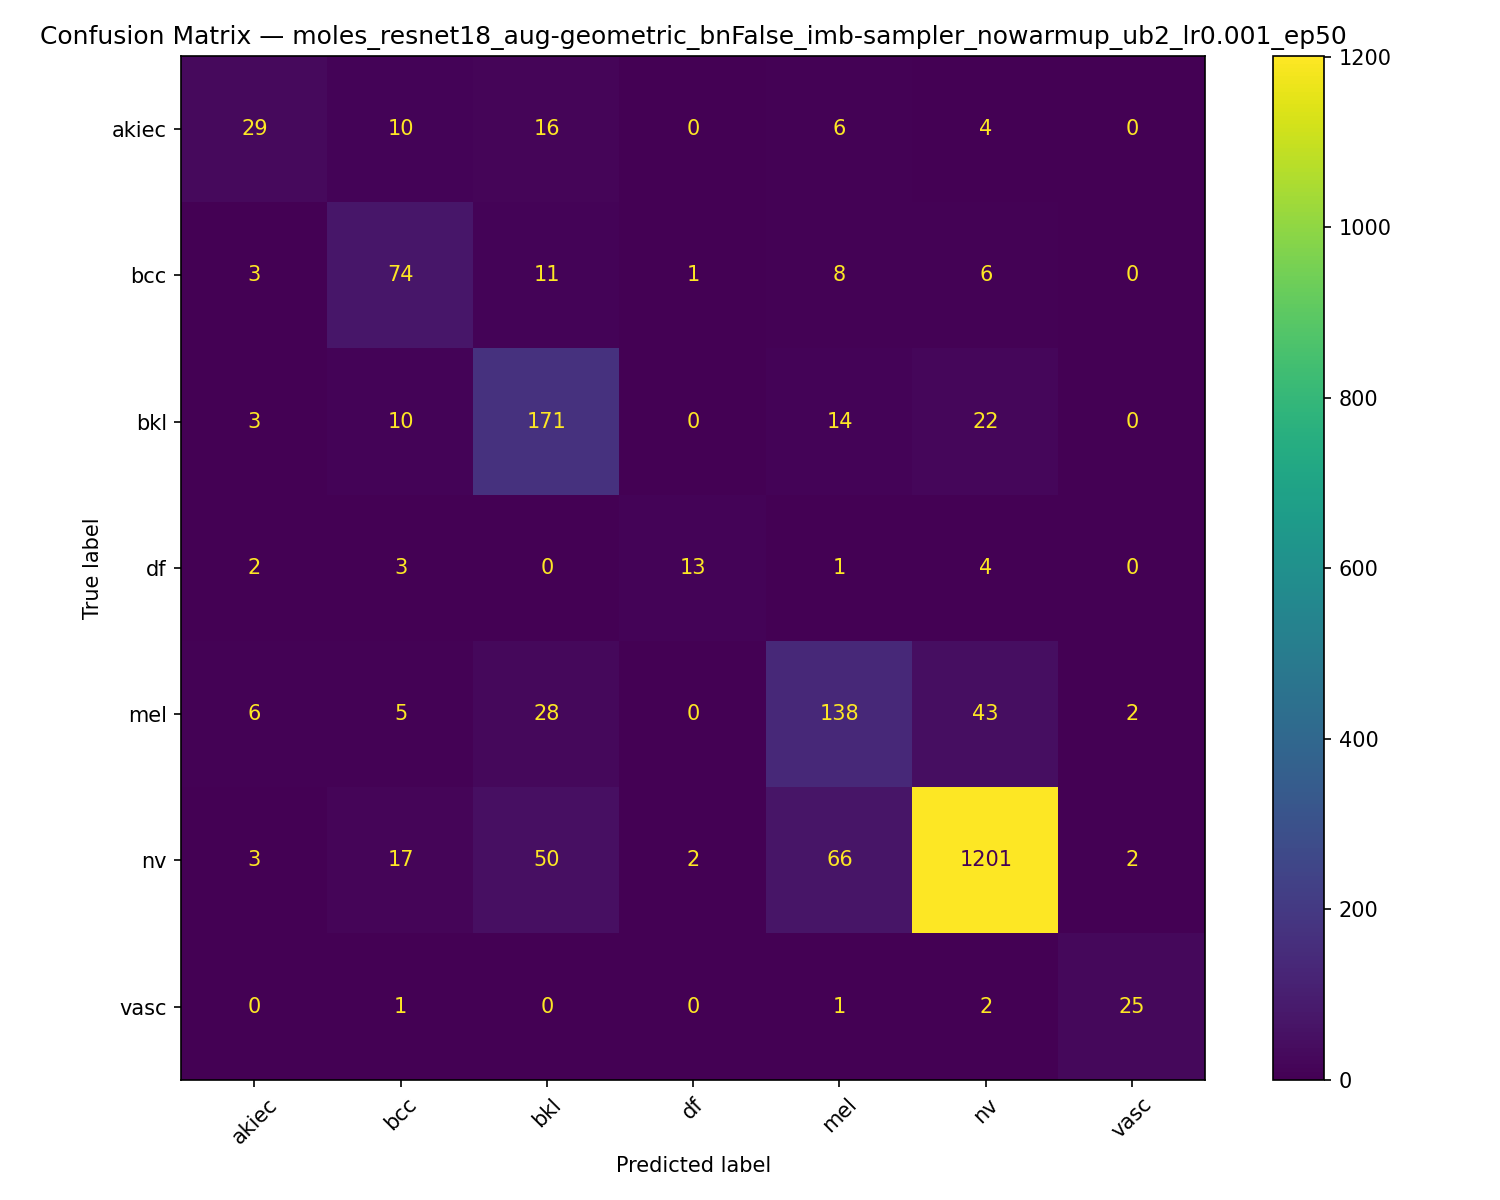
\includegraphics[width=0.48\textwidth]{graphs/moles_resnet18_aug-geometric_bnFalse_imb-sampler_nowarmup_ub2_lr0.001_ep50_confusion_matrix.png}
\hfill
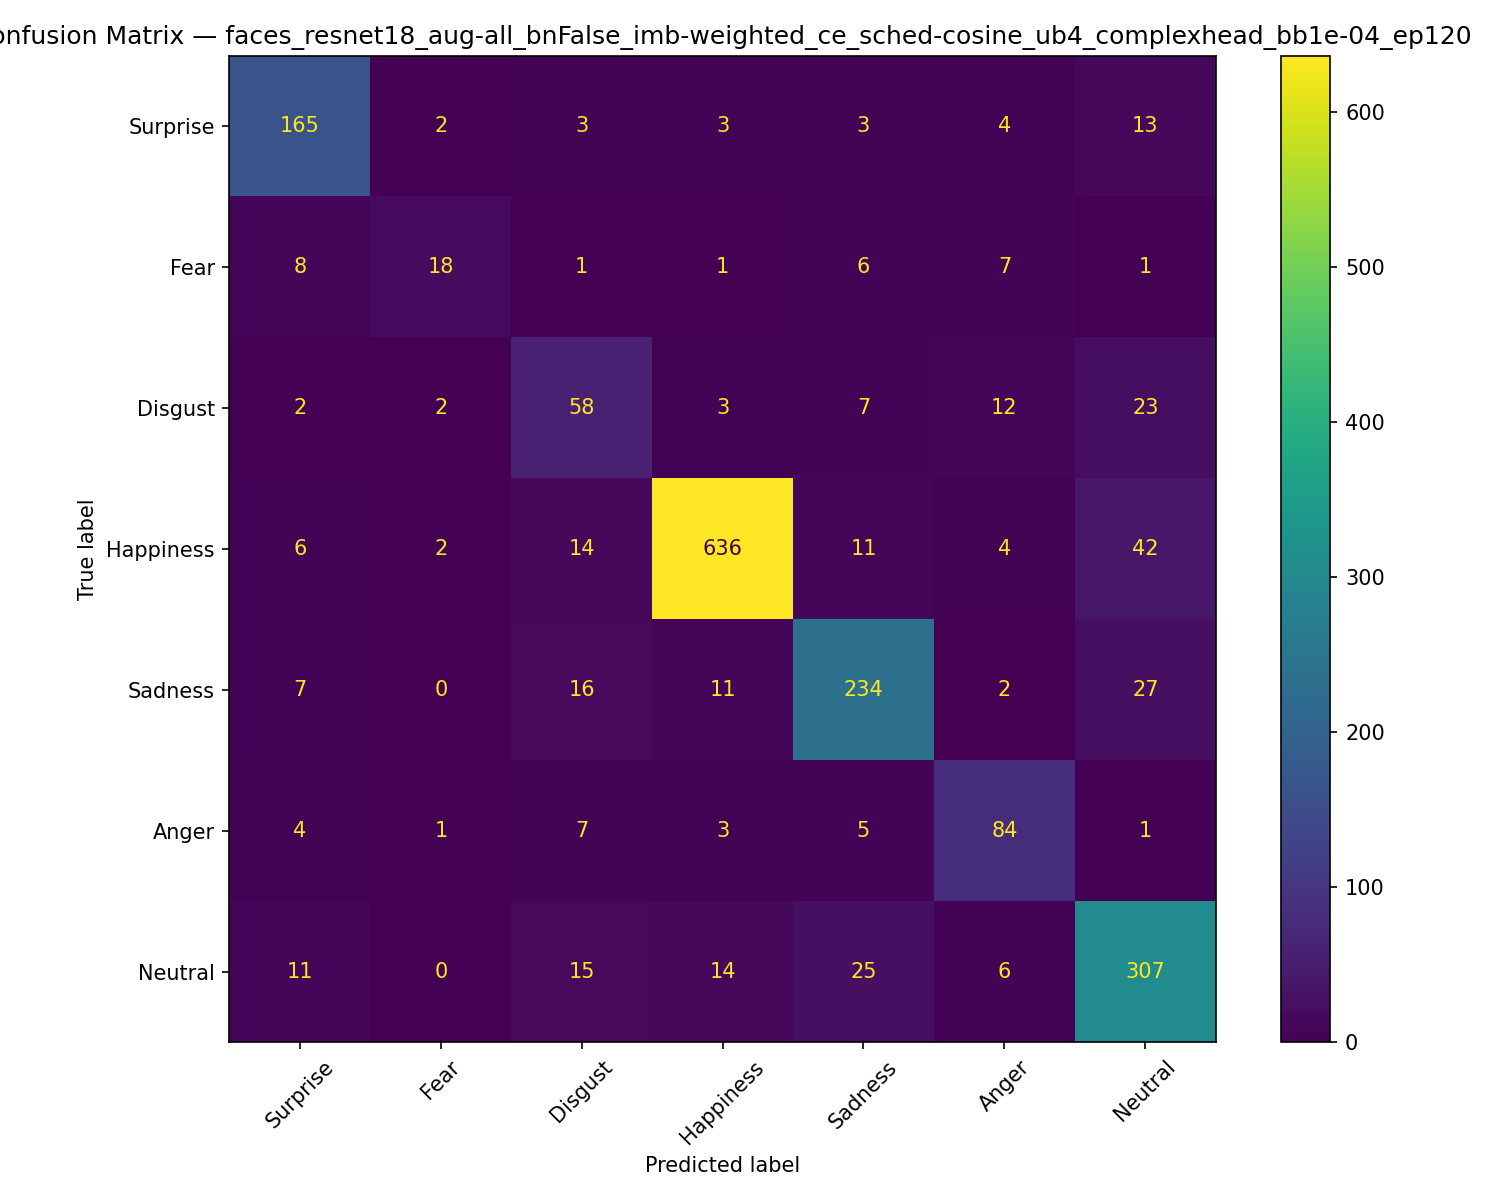
\includegraphics[width=0.48\textwidth]{graphs/faces_resnet18_aug-all_bnFalse_imb-weighted_ce_sched-cosine_ub4_complexhead_bb1e-04_ep120_confusion_matrix.png}
\caption{Matricele de confuzie finale: Moles (stânga) și Faces (dreapta)}
\label{fig:confusion_matrices}
\end{figure}

Pe setul \texttt{Moles}, utilizând \texttt{ResNet-18} (Scenariul 2, cu sampler, fără warmup), s-au obținut următoarele metrici finale de performanță:
\begin{itemize}
    \item \textbf{Acuratețe / F1-Micro:} 84.32\%
    \item \textbf{F1-Macro:} 0.7267
\end{itemize}
Matricea de confuzie evidențiază o recunoaștere corectă a clasei majoritare \texttt{nv} (1124 din 1341 mostre), dar și o performanță ridicată pe clasele minoritare datorită utilizării samplerului echilibrat.

Pe setul \texttt{Faces}, utilizând \texttt{ResNet-18} (120 de epoci, standard run), s-au obținut următoarele metrici finale de performanță:
\begin{itemize}
    \item \textbf{Acuratețe / F1-Micro:} 82.04\%
    \item \textbf{F1-Macro:} 0.7408
\end{itemize}
Matricea de confuzie confirmă o generalizare echilibrată a emotiilor dificile (de exemplu, frica sau dezgustul), reducând semnificativ erorile pe clasele minoritare.

\end{document}